% !TeX root = ./principal.tex
% Modelo de Tese/Dissertação para UNIFEI
\documentclass[
    % opções da classe memoir
    12pt,
    oneside,
    a4paper,
    oldfontcommands,
    % opções do pacote babel
    english,			% idioma adicional para hifenização
    brazil				% o último idioma é o principal do documento
    ]{abntex2} 
    
    % configurações (pacotes, comandos)
    % Pacotes fundamentais 
\usepackage[brazil]{babel}
\usepackage{cmap}			    % Mapear caracteres especiais no PDF
\usepackage{lmodern}			% Usa a fonte Latin Modern			
\usepackage[T1]{fontenc}		% Selecao de codigos de fonte.
\usepackage[utf8]{inputenc}		% Codificacao do documento (conversão automática dos acentos)
\usepackage{lastpage}			% Usado pela Ficha catalográfica
\DisemulatePackage{setspace}
\usepackage{setspace}
\usepackage{indentfirst}		% Indenta o primeiro parágrafo de cada seção.
\usepackage{color}			    % Controle das cores
\usepackage{graphicx}			% Inclusão de gráficos
\usepackage{pdfpages}
\usepackage{bmpsize}
\usepackage[cmex10]{amsmath}	% Formulas matemáticas
\usepackage{amsfonts,amssymb,latexsym}
\usepackage{mathtools}
\usepackage{bigints}
%\usepackage{amscls}
\usepackage{subfig}
\usepackage[siunitx]{circuitikz}
%\usepackage{booktabs}
%\usepackage{longtable}
%\usepackage{tabularx}
\usepackage{array}
\usepackage{multirow}
\usepackage{pgfplots}
%\pgfplotsset{compat=1.14}
\pgfplotsset{compat=newest}
%\usepackage{geometry} 			% Fazer uma pagina em retrato
\usepackage{pdflscape}
\usepackage{nomencl}
\makenomenclature
\usepackage{textcase}
\usepackage{colortbl}
\usepackage[normalem]{ulem}
\usepackage{tikz}

% acrônimos e símbolos usando o pacote glossaries
\usepackage{hyperref}
\usepackage[symbols,acronym,nopostdot,nogroupskip,indexonlyfirst]{glossaries}
\setacronymstyle{short-long}
\setlength{\glsdescwidth}{0.8\textwidth}
\setlength{\glspagelistwidth}{0.2\textwidth}
\loadglsentries[\acronymtype]{siglas}
\loadglsentries[symbols]{simbolos}
\makeglossaries

\usepackage{anyfontsize}

% Pacotes adicionais, usados apenas no âmbito do Modelo Canônico do abnteX2
\usepackage{lipsum}				% para geração de dummy text

% Pacotes de citações
\usepackage[brazilian,hyperpageref]{backref}	% Paginas com as citações na bibl
\usepackage[alf, bibjustif]{abntex2cite}		% Citações padrão ABNT: usar alf ou num
\citebrackets()
\hyphenation{di-mi-nu-i-ção}
\hyphenation{ha-lo-im-plan-ta-dos}

% CONFIGURAÇÕES DE PACOTES
% Configurações do pacote backref
% Usado sem a opção hyperpageref de backref
%\renewcommand{\backrefpagesname}{Citado na(s) página(s):~}
% Texto padrão antes do número das páginas
%\renewcommand{\backref}{}
% Define os textos da citação
%\renewcommand*{\backrefalt}[4]{
%	\ifcase #1 %
%		Nenhuma citação no texto.%
%	\or
%		Citado na página #2.%
%	\else
%		Citado #1 vezes nas páginas #2.%
%	\fi}%

% Configurações de aparência do PDF final
% alterando o aspecto da cor azul
\definecolor{blue}{RGB}{0,0,192}

% informações do PDF
\makeatletter
\hypersetup{
     	%pagebackref=true,
		pdftitle={\@title}, 
		pdfauthor={\@author},
    	pdfsubject={\imprimirpreambulo},
	    pdfcreator={LaTeX with abnTeX2},
		pdfkeywords={abnt}{latex}{abntex}{abntex2}{trabalho acadêmico}, 
		colorlinks=true,       		% false: boxed links; true: colored links
    	linkcolor=blue,          	% color of internal links
    	citecolor=blue,        		% color of links to bibliography
    	filecolor=magenta,      	% color of file links
		urlcolor=blue,
		bookmarksdepth=4
}
\makeatother

% Espaçamentos entre linhas e parágrafos 
% Retira espaço extra obsoleto entre as frases.
\frenchspacing 

% O tamanho do parágrafo é dado por:
\setlength{\parindent}{1.3cm}

% Controle do espaçamento entre um parágrafo e outro:
\setlength{\parskip}{0.2cm}  % tente também \onelineskip

% compila o indice
\makeindex

% comandos úteis
\newcommand{\cmmt}[1]{} % comenta trecho de um parágrafo. Ex.: ..texto \cmmt{texto a ser comentado} texto..
\newcommand{\mat}[1]{\mathbf{#1}}
\def\H{^{\mathrm{H}}}
\def\T{^{\mathrm{T}}}

%\usepackage{showframe}% added to show that the figure is being centered
    % informações (título, autor, instituição, banca examinadora, etc.)
    % Informações de dados para CAPA e FOLHA DE ROSTO

\titulo{Uma ferramenta colaborativa para evolução de uma taxonomia}
\autor{Mário Guilherme Macedo}
\local{Itajubá}
\data{\today}
\orientador{Prof.\textsuperscript{a} Dr.\textsuperscript{a} Melise Maria Veiga de Paula}
\coorientador{Prof. Dr. Coorientador}
\instituicao{Universidade Federal de Itajubá - UNIFEI}
\def \siglaInstituicao{UNIFEI}
\def \orientadorTexto{Monografia realizada sob orientação da \imprimirorientador}
\def \programaLinhaUm{}
\def \programaLinhaDois{}
\def \programa{\programaLinhaUm \space \programaLinhaDois}
\def \areaconcentracao{Área de Concentração: Microeletrônica}

%\tipotrabalho{Tese (Doutorado)}
\tipotrabalho{Trabalho Final de Graduação}

% O preambulo deve conter o tipo do trabalho, o objetivo, o nome da instituição e a área de concentração 
\preambulo{Monografia apresentada como trabalho final de graduação, requisito parcial para obtenção do título de Bacharel em Ciência da Computação, sob orientação da \imprimirorientador.}

% aprovação
\def \diadeaprovacao{23}
\def \mesdeaprovacao{Outubro}
\def \anodeaprovacao{2018}

% frase utilizada na folha de aprovação
\def  \aprovacao{\large Dissertação aprovada por banca examinadora em \diadeaprovacao \space de \mesdeaprovacao \space de \anodeaprovacao, conferindo ao autor o título de \textbf {Mestre em Ciências em Engenharia Elétrica.}}

% Banca examinadora - Professores convidados
\def \professorConvidadoUm{Membro da Banca Examinadora}
\def \professorConvidadoDois{Prof.\textsuperscript{a} Dr.\textsuperscript{a} Isabela Neves Drummond}
\def \professorConvidadoTres{Prof. Dr. Convidado3}
\def \professorConvidadoQuatro{Prof. Dr. Convidado4}
\def \professorConvidadoCinco{Prof. Dr. Convidado5}

% Banca examinadora
\def \bancaexaminadora{\professorConvidadoUm \\ \professorConvidadoDois \\ \professorConvidadoTres \\ \professorConvidadoQuatro \\ \professorConvidadoCinco}
    
    % Início do documento
    \begin{document}
    
    % Elementos pré-textuais
    % Capa
    % Capa
%\imprimircapa
\begin{center}
    {\large \textbf{\MakeUppercase{\imprimirinstituicao}}}\\[1.5cm]

    
\includegraphics[width=25mm,height=25mm,scale=0.5]{./figuras/efei.png}\\[5cm]

    {\large \textbf{\textrm{\MakeUppercase{\imprimirtitulo}}}}\\[5cm]

    \begin{flushright}
        {\large \textrm{\imprimirautor}} \\[2cm]
    \end{flushright}

    \vfill
    \large \siglaInstituicao \\ \imprimirlocal \\ \anodeaprovacao
\end{center}
\newpage
    % Folha de Rosto
    \vfill
	\begin{center}
		{\large \textbf{\MakeUppercase{\imprimirinstituicao}}}\\[2cm]

		{\large \textbf{\imprimirautor}}\\[4cm]

		{\large \textbf{\textrm{\MakeUppercase{\imprimirtitulo}}}}\\[4cm]
		\hspace{7cm} %posicionamento da mini página do titulo
		\begin{minipage}{.5\textwidth}		
			\begin{flushleft}
				\imprimirpreambulo
			\end{flushleft}	
		\end{minipage}
		\vfill
		\large \siglaInstituicao \\ \imprimirlocal \\ \anodeaprovacao
	\end{center}
    \newpage
    % Folha de Aprovação 1
    %% Isto é um exemplo de Folha de aprovação, elemento obrigatório da NBR
% 14724/2011 (seção 4.2.1.3). Você pode utilizar este modelo até a aprovação
% do trabalho. Após isso, substitua todo o conteúdo deste arquivo por uma
% imagem da página assinada pela banca com o comando abaixo:
%
% \includepdf{folhadeaprovacao_final.pdf}
%
\begin{folhadeaprovacao}
\vfill

\begin{center}
{\large \textbf{\MakeUppercase{\imprimirinstituicao}}}\\
{\large \textbf{\MakeUppercase{\programaLinhaUm}}}\\
{\large \textbf{\MakeUppercase{\programaLinhaDois}}}\\[3cm]
{\Huge \imprimirtitulo.}\\[3cm]
{\large \textbf{\imprimirautor}} \\[1cm]

\end{center}
\vfill
\begin{flushright}
\begin{minipage}{11cm}
{
	% frase da aprovação, editar o arquivo "info.tex" para alterar
	\aprovacao
}\\[1cm]
\end{minipage}
\end{flushright}

	\begin{flushright}
	\begin{minipage}{11cm}
		\textit{\large \textbf{Banca Examinadora:\\}}
			{\large \bancaexaminadora}
	\end{minipage}
	\end{flushright}
\begin{center}
	\large \textbf{\imprimirlocal}\\
	\large \textbf{\anodeaprovacao}
\end{center}
\end{folhadeaprovacao}
\newpage
    % Ficha Catalográfica
    %% Isto é um exemplo de Ficha Catalográfica, ou "Dados internacionais de catalogação-na-publicação''. Você pode utilizar este modelo como referência.  Porém, provavelmente a biblioteca da sua universidade lhe fornecerá um PDF com a ficha catalográfica definitiva após a defesa do trabalho. Quando estiver com o documento, salve-o como PDF no diretório do seu projeto e substitua todo o conteúdo de implementação deste arquivo pelo comando abaixo:
% \begin{fichacatalografica}
%     \includepdf{fig_ficha_catalografica.pdf}
% \end{fichacatalografica}

\begin{fichacatalografica}
	\vspace*{\fill}					% Posição vertical
	\hrule							% Linha horizontal
	\begin{center}					% Minipage Centralizado
	\begin{minipage}[c]{12.5cm}		% Largura
	
	\imprimirautor
	
	\hspace{0.5cm} \imprimirtitulo  / \imprimirautor. --
	\imprimirlocal, \imprimirdata-
	
	\hspace{0.5cm} \pageref{LastPage} p. : il. (algumas color.) ; 30 cm.\\
	
	\hspace{0.5cm} \imprimirorientadorRotulo~\imprimirorientador\\
	
	\hspace{0.5cm}
	\parbox[t]{\textwidth}{\imprimirtipotrabalho \\\imprimirinstituicao\\ \programa, \imprimirdata.}\\
	
	\hspace{0.5cm}
		1. Palavra-chave1.
		2. Palavra-chave2.
		I. Orientador.
		II. Universidade xxx.
		III. Faculdade de xxx.
		IV. Título\\ 			
	
	\hspace{8.75cm} CDU 07:181:009.3\\
	
	\end{minipage}
	\end{center}
	\hrule
\end{fichacatalografica}
    % Folha de Aprovação 2
    % Isto é um exemplo de Folha de aprovação, elemento obrigatório da NBR
% 14724/2011 (seção 4.2.1.3). Você pode utilizar este modelo até a aprovação
% do trabalho. Após isso, substitua todo o conteúdo deste arquivo por uma
% imagem da página assinada pela banca com o comando abaixo:
%
% \includepdf{folhadeaprovacao_final.pdf}
%
\begin{folhadeaprovacao}
  \begin{center}
    {\large \textbf{\MakeUppercase{\imprimirinstituicao}}}\\[2cm]
    {\large \textbf{\textrm{\MakeUppercase{\imprimirtitulo}}}}\\[2cm]
    \begin{flushright}
      {\ABNTEXchapterfont\large \textrm{\imprimirautor}}
    \end{flushright}   

    \vspace{2cm}
    \begin{minipage}{1\textwidth}
      \doublespacing
      Esta monografia parcial foi julgada e aprovada como requisito parcial para obtenção do título de Bacharel em Ciência da Computação,
      sob orientação da \orientador.\\

      \imprimirlocal, \today.
    \end{minipage}%
    \vspace*{\fill}
   \end{center}
    
\assinatura{\imprimirorientador\\ Orientadora} 
\assinatura{\professorConvidadoUm}
\assinatura{\professorConvidadoDois\\ Coordenadora do TFG}

\begin{center}
  \vfill
  \large \siglaInstituicao \\ \imprimirlocal \\ \anodeaprovacao
\end{center}

\end{folhadeaprovacao}
\newpage
    % Epígrafe
    \begin{epigrafe}
    \vspace*{\fill}
	\begin{flushright}
	\textit{"It takes considerable knowledge just to realize the extent of your own ignorance."\\
		(Dr. Thomas Sowell)}
	\end{flushright}
\end{epigrafe}
\newpage
    % Agradecimentos
    %\begin{agradecimentos}
Agradeço a Deus ...
\end{agradecimentos}
\newpage
    % Resumo
    \newpage
% resumo em português
\begin{resumo}
O número de iniciativas de participação com o objetivo de estreitar a distância entre governos e cidadãos têm aumentado. 
Os conceitos de governança digital, governo eletrônico e participação eletrônica entraram na agenda de grandes organizações 
que buscam o desenvolvimento da sociedade. Nesse contexto, a utilização de ferramentas de participação eletrônica têm se tornado um 
grande meio para fiscalizar governos, compartilhar dados e resolver as demandas da sociedade.
Alinhado a isso, o objetivo desse trabalho é desenvolver uma aplicação \textit{web}, denominada e-TAPE, para apoiar a edição 
colaborativa de uma taxonomia sobre ferramentas de participação eletrônica. A proposta é que a e-TAPE facilite a interação dos usuários 
de maneira intuitiva e amigável e funcione como um canal para que, tanto pesquisadores quanto potenciais usuários de ferramentas de 
participação eletrônica, colaborem para evolução da taxonomia. Na e-TAPE, os usuários têm acesso à taxonomia e às ferramentas de 
participação eletrônica já classificadas. A usabilidade da e-TAPE é avaliada, seguindo metodologias já validadas no meio acadêmico e
os resultados indicam que a e-TAPE possui um bom indicador de usabilidade perante aos usuários que realizaram o teste. 

\noindent
 \textbf{Palavras-chaves}: Taxonomia, participação eletrônica, ferramentas de participação eletrônica, TAPE, e-TAPE, governo eletrônico e governança digital.
\end{resumo}
\newpage
    % Resumo em inglês
    \begin{resumo}[Abstract]
 \begin{otherlanguage*}{english}
 
 This work presents ...
 
   \vspace{\onelineskip}
 
   \noindent 
   \textbf{Key-words}: ABC. DEF. GHF.
 \end{otherlanguage*}
\end{resumo}
\newpage
    % Sumário
    \pdfbookmark[0]{\contentsname}{toc}
\tableofcontents*
\cleardoublepage
    % Lista de ilustrações
    \pdfbookmark[0]{\listfigurename}{lof}
\listoffigures*
\cleardoublepage
    % Lista de tabelas
    \pdfbookmark[0]{\listtablename}{lot}
\listoftables*
\cleardoublepage
    % Lista de abreviaturas e siglas
    % inserir lista de siglas
\renewcommand{\nomname}{\listadesiglasname}
\pdfbookmark[0]{\nomname}{loa}
\cleardoublepage
\printglossary[title=\ABNTEXchapterfont\ABNTEXchapterfontsize\listadesiglasname,type=\acronymtype,style=long3col]
\pagebreak
    % Lista de símbolos
    % inserir lista de símbolos
\renewcommand{\nomname}{\listadesimbolosname}
\pdfbookmark[0]{\nomname}{los}
\cleardoublepage
\printglossary[title=\ABNTEXchapterfont\ABNTEXchapterfontsize\listadesimbolosname,type=symbols,style=long3col]
\pagebreak
    
    % Elementos textuais
    \textual
    % Capítulos
    % Capítulo 1 - Introdução
    \chapter[Introdução]{Introdução}
\label{cap:cap1}
Uma tendência que vem sendo observada é a aproximação entre os cidadãos e seus governantes, um exemplo disso são as iniciativas de governos abertos.
A agenda de 2030 da \acrfull{onu} para a transformação do mundo através do desenvolvimento sustentável deixa claro, no parágrafo 48, que
indicadores estão sendo desenvolvidos para ajudar a estreitar a distância entre governo e cidadão. Dados acessíveis, atualizados e confiáveis serão necessários para colaborar 
com a análise do progresso das iniciativas sobre participação. 
Esses dados são de suma importância para a tomada de decisão \cite{assembly2015transforming}.

\par
A \acrshort{onu} define o conceito de participação eletrônica como o processo de engajar cidadãos através de \acrfull{tic} em política, tomadas de decisão e
serviços públicos, fazendo com que este processo seja inclusivo, participativo e deliberado. Em \citeonline{braga2016participaccao}, os autores mostram que o uso de 
ferramentas de participação eletrônica tornou-se fundamental para o cumprimento das metas traçadas pela agenda da \acrshort{onu} em 2015. 

\par
Isso dá-se pelo fato de que a utilização de \acrshort{tic} pelo setor público tem transformado a governança global, exigindo que os agentes públicos forneçam melhores serviços 
de maneira eficiente e barata \cite{afdb2014uneca}. 

\par
Esse tipo de demanda provoca a adoção, pelo poder público, de infraestruturas tecnológicas para a melhorar a eficácia ao ofertar serviços à população. Esse conceito é interpretado
por \citeonline{reddick2012public} como governança digital, ou seja, governança digital é a melhora da capacidade do Estado em fazer uso de tecnologias e da internet 
para a implementação de suas políticas.

\par
A \acrfull{ocde}, juntamente com a \acrshort{onu} e a \acrfull{ue}, criaram \textit{frameworks} para a avaliação do \textit{status} da governança digital através de indicadores \cite{onu2018}. A metodologia utilizada permite medir a eficácia na prestação de serviços públicos e identificar padrões de desenvolvimento e desempenho. Um dos aspectos analisados são as oportunidades oferecidas pela gestão através da participação eletrônica. 
Atualmente, governantes podem encontrar diretrizes para desenvolver esse tipo de ferramenta de forma mais apropriada.
Por exemplo,  no trabalho de \citeonline{scherer2010hands}, os autores apresentam uma metodologia para a criação de duas ferramentas de participação eletrônica na Europa, a VoicE e a VoiceS.

\par
Outra vertente de estudo nessa área tem sido o esforço de classificação de ferramentas de participação eletrônica. Em  \citeonline{kinyik2015guideline}, o autor apresenta um modelo 
de classificação elaborado no contexto do projeto \acrfull{e-uropa} cujo objetivo é aumentar e disseminar o conhecimento dos cidadãos europeus sobre ferramentas de participação 
eletrônica, alegando que as demandas da sociedade seriam melhores e mais rapidamente atendidas. Contudo, apesar dos esforços de classificação, o conhecimento a respeito desse 
tipo de ferramenta ainda é restrito. Dessa forma, é necessário a elaboração de estratégias que possam popularizar ou ampliar o alcance dessas iniciativas perante a sociedade.

\par
Alinhado a essa necessidade, o objetivo desse trabalho é desenvolver uma aplicação \textit{web}, denominada e-TAPE, para apoiar a edição colaborativa de uma taxonomia sobre 
ferramentas de participação eletrônica. O nome atribuído à taxonomia, que é base para ferramenta, é \acrfull{tape}, nome dado pelos autores \citeonline{tape2019mota}. 
A proposta é que a e-TAPE facilite a interação dos usuários de maneira intuitiva e amigável e funcione como um canal para que, tanto pesquisadores quanto potenciais usuários de
ferramentas de participação eletrônica, colaborem para evolução da taxonomia. Na e-TAPE, os usuários têm acesso à taxonomia e às ferramentas de participação eletrônica já classificadas.


\par
É esperado que a ferramenta contribua tanto para a pesquisa quanto para a prática do assunto abordado. No que diz respeito à pesquisa, a e-TAPE pode ajudar os pesquisadores a entender mais sobre domínio estudado. Além disso, a utilização de um modelo sistemático representado pela taxonomia 
pode facilitar a identificação dos pontos fortes e fracos do domínio, criando novas possibilidades de investigação. Por outro lado, tanto para o gestor público, quanto para o cidadão comum, 
o uso da e-TAPE pode facilitar a escolha de ferramentas de participação eletrônica que se adéquem mais ao seu contexto. Essa escolha poderá levar em conta critérios 
isolados ou uma combinação de critérios, dependendo da demanda. 

\par
A usabilidade da e-TAPE foi avaliada seguindo metodologias já validadas no meio acadêmico, como os trabalhos de \citeonline{brooke1996sus} e \citeonline{sauro2015supr}. Os resultados indicaram que a e-TAPE apresentou uma usabilidade apropriada, embora tenha sido identificada a necessidade de alguns ajustes. 

\par
O texto está organizado da seguinte forma: no Capítulo \ref{cap:cap2}, é apresentada a revisão da literatura considerando os principais conceitos necessários a uma melhor 
compreensão do trabalho. No capítulo \ref{cap:cap3}, é descrita metodologia adotada para o desenvolvimento da aplicação e outros aspectos relacionados à e-TAPE como funcionalidades e recursos tecnológicos utilizados. Já no capítulo \ref{cap:cap4}, é descrita avaliação de usabilidade e os resultados obtidos. 
A conclusão e as sugestões para futuros trabalhos encontram-se no capítulo \ref{cap:cap5}.

    % Capítulo 2 - Revisão Bibliográfica
    \chapter[Revisão Bibliográfica]{Revisão Bibliográfica} 
\label{cap:cap2}
%Eu acho que você quis associar o conceito de participação com governança e transparência, acho essa abordagem muito legal. 
%Mas acho que falta você trabalhar um pouco mais essa relação. Pensa que deve existir uma coerência nessa discussão:
%minha sugestão é que você desenvolva melhor o texto seguindo esse caminho: governança digital->transparência->participação

% Introdução do capítulo
Neste capítulo serão discutidos alguns aspectos teóricos necessários para uma boa compreensão do desenvolvimento deste trabalho.

% 1a seção do capítulo 1
\section{Participação Eletrônica e Governança Digital}
\label{sec:e-part}
\par
A utilização de \acrshort{tic} pelo setor público tem transformado a governança global, exigindo de governos e governantes o fornecimento de serviços melhores, 
mais econômicos e eficientes às organizações e indivíduos \cite{afdb2014uneca}. Fatores como o reconhecimento da sociedade civil organizada, o aumento da participação cidadã e a 
ampliação e diversificação dos temas abordados nas esferas governamentais determinaram um novo modelo de governança, a governança digital \cite{o2011government}. 
Este modelo acaba por oferecer um espaço, antes não existente, onde o uso inovador das \acrshort{tic} é a principal ferramenta para ampliar a transparência e participação.

\par
A noção de governança digital é interpretada por \citeonline{reddick2012public} como o resultado da adoção de infraestruturas tecnológicas para a otimização da entrega de 
serviços à população. Ou seja, a utilização de \acrshort{tic} pelo setor público passa a se referir ao modo como as tecnologias e a internet podem melhorar a capacidade do Estado 
de formular e implementar suas políticas públicas \cite{parra2017governancca}. \citeonline{germani2016desafios} complementa a definição de governança digital afirmando que sua 
utilização pelo setor público deve ter o objetivo de melhorar a disponibilização de informações e o fornecimento de serviços públicos aos cidadãos, 
além de incentivar o engajamento da sociedade nos processos políticos, aprimorando os níveis de responsabilidade, transparência e efetividade do governo.

\par
De acordo com o conceito de governança digital apresentado pela \acrshort{onu}, o uso de \acrshort{tic} deve ser definido para atender aos três pilares fundamentais: 
a prestação de melhores serviços pelos agentes públicos, o maior acesso à informação e a maior participação da sociedade civil em todos os ciclos de políticas públicas. 
Dessa forma, as \acrshort{tic} representam o papel de viabilizadoras desses três pilares podendo obter níveis de desempenho mais satisfatórios \cite{onu2018}. 

\par
Para \citeonline{rushkoff2003open}, o conceito de governança digital democratiza a tomada de decisão e incentiva a colaboração voluntária entre os indivíduos. Para \citeonline{braga2016participaccao} a possibilidade de um maior acesso às informações e ao conhecimento permite uma maior transparência nas decisões tomadas por governantes. Diversos paradigmas sobre este modelo de tomada de decisão vêm sendo reexaminados. Além disso, o papel do gestor público e do cidadão têm sido reavaliados pois a incorporação 
de novas tecnologias na relação entre estado e sociedade amplia e possibilita uma outra dinâmica a essa relação. 

\par
Em \citeonline{vaz2017transformaccoes}, o autor apresenta uma nova perspectiva: o aumento da comunidade \textit{open source} atrelado à difusão dos dados abertos governamentais tem permitido a produção descentralizada de aplicações, serviços e sistemas tecnológicos. Criando assim, o que o autor chama de Segunda Geração de Governança Digital, 
que consiste na busca por iniciativas além das unidirecionais, nas quais o governo apenas disponibiliza os dados captados sobre a população.

\par

\citeonline{vaz2017transformaccoes} argumenta que há a necessidade de alteração do atual modelo \textit{broadcasting}, para um modelo mais participativo de tomada de decisões. 
O autor define "modelo \textit{broadcasting}" como um modelo de alocação dos recursos digitais como recursos secundários ou complementares 
às iniciativas presenciais de relacionamento entre governos e sociedade. Nesse modo, são os governantes que estabelecem os momentos, formatos e conteúdo dos processos 
participativos e de controle social. Isso acaba por restringir as iniciativas apenas às iniciativas governamentais, nas quais a interação e participação nas decisões e no
controle social das políticas públicas são monopolizadas pelo Estado \cite{parra2017governancca}.

\par
Para que haja a evolução desse modelo atual, \citeonline{o2011government} sugere que o governo deve disponibilizar suas informações em uma infraestrutura que permita a reutilização
sistemática pela sociedade civil. Ao disponibilizar suas informação, o governo estimula o desenvolvimento de inciativas e ferramentas tecnológicas, ampliando assim a possibilidade 
do uso diverso das informações \cite{zuiderwijk2012socio}. As funções de fazer política e entregar serviços públicos precisam ser reinterpretadas e a participação dos cidadãos
tem que se dar de uma maneira mais ativa \cite{bovaird2007beyond}, um exemplo de iniciativa popular que corrobora com essa ideia é o Serenata de Amor.

\par
Serenata de Amor é um projeto aberto com o objetivo de aumentar a fiscalização dos gastos públicos, compartilhando-os de maneira clara e acessível para a sociedade. O projeto utiliza
aprendizado de máquina para fiscalizar os reembolsos efetuados pela \acrfull{ceap} - verba que custeia alimentação, transporte, hospedagem e até despesas com cultura e 
assinaturas de TV dos parlamentares brasileiros. \textit{Serenata de Amor}. Disponível em: <https://serenata.ai/>. Acesso em 03 out. 2018.


\par
De acordo com a \citeonline{onu2018}, promover essa participação cidadã é fundamental para a governança de uma sociedade civil organizada e inclusiva. O objetivo dessa governança deve
ser direcionado à melhoraria do acesso às informações e aos serviços públicos, pelo incentivo à inclusão do cidadão na tomada de decisões públicas que impactem o bem estar da 
sociedade e do indivíduo em particular.  Neste contexto, surge o conceito de Participação Eletrônica definido por \citeonline{macintosh2008democracy} como o uso de \acrshort{tic}
a fim de ampliar e aprofundar a participação política para que cidadãos sejam capazes de se conectar uns aos outros e aos seus representantes eleitos. 

\par 
De acordo com \cite{medeiros2009novos}, o uso das ferramentas de participação eletrônica tem se disseminado e vem sendo aplicado a diversos objetivos e ambientes diferentes, podendo 
ser encontrados exemplos por todo o mundo. \citeonline{dal2015ferramentas}, por exemplo, mostra em sua pesquisa exploratória sobre inciativas destinadas à participação civil
pela internet, casos de uso de ferramentas de participação eletrônica em Barcelona, Lisboa, São Paulo, Nova Iorque e Porto Alegre. A autora chega a conclusão 
que o uso de ferramentas de participação eletrônica por governos é um "caminho sem volta".%TODO: Citar artigo

\par
Contudo, a sociedade civil ainda não tem se engajado plenamente ao uso desses recursos. Para exemplificar, temas de grande interesse popular 
como as reformas trabalhista, tributária e da previdência social brasileira recebem grande atenção dos veículos de comunicação sendo relatados por especialistas como fundamentais 
para o desenvolvimento do país. Portanto, é razoável esperar que que os cidadãos se sintam motivados à participar de discussões voltadas a esses temas. 
Contudo, a ferramenta de participação eletrônica Wikilegis, desenvolvida pela câmara dos deputados do Brasil, disponibilizada em um ambiente virtual onde a sociedade civil pode analisar
 os projetos de leis e contribuir com sugestões para redação aos artigos ou parágrafos, apresenta uma quantidade inexpressiva de sugestões para os projetos de reformas. 
 São 221 sugestões para a reforma da previdência, 129 sugestões para a reforma tributária e  50 sugestões para a reforma trabalhista.  Os números mostram a dificuldade de engajar 
 a sociedade civil em assuntos políticos mais complexos e que demandam tempo e estudo. \textit{Wikilegis}. Disponível em <https://edemocracia.camara.leg.br>. Acesso em 10 out 2018. 

\par
Por outro lado, durante a pesquisa, foi possível encontrar casos onde o engajamento dos cidadãos foi maior. Por exemplo, o site Vote na web disponibiliza um painel, onde são mostrados projetos de leis, 
seus propositores e componentes gráficos para representar a votação dos cidadãos.
Assim, o cidadão pode comparar sua intenção de voto com as dos demais cidadãos e com os votos efetivados pelos representantes, além de contar com a descrição dos votos por gênero,
região e idade. Os projetos têm em média sete mil votos, onde o mais votado conta com cerca de quase quinze mil votos. \textit{Vote na Web}. Disponível em <http://www.votenaweb.com.br/>.
Acesso em 10 out 2018.

\par
Isso indica que o engajamento da sociedade civil organizada tem um amplo espaço de crescimento \cite{o2011government}, fica o desafio aos atores, sociedade civil, governantes, 
empresas e indivíduos, a criação de ferramentas de participação eletrônica que estimulem o engajamento do cidadão.


%=====================================================================================================================================================================================================
% FERRAMENTAS DE PARTICIPAÇÃO ELETRÔNICA
%=====================================================================================================================================================================================================

\section{Ferramentas de Participação Eletrônica}
\label{sec:e-part tools}
Devido aos incentivos gerados por esses novos paradigmas de tomada de decisões participativas, muitas ferramentas de participação eletrônica têm sido desenvolvidas,
tanto por governos e governantes, quanto pela sociedade civil organizada. Alguns exemplos de ferramentas de participação eletrônica identificados podem ser encontrados na Tabela \ref{tab:ferramentas}.

\vspace{1cm}

\begin{table}[!ht]
    \centering
    \caption{Ferramentas de Participação Eletrônica}
    \label{tab:ferramentas}
    \begin{tabular}{l*{2}{>{\raggedright\arraybackslash}p{0.5\linewidth}}}
    \toprule
        Nome                             & Acesso                           \\ 
    \midrule
        Crowd For Roads                  & c4rs.eu                          \\
        Decidim Barcelona                & decidim.barcelona                \\
        e-Cidadania                      & senado.leg.br/ecidadania         \\
        Iniciativa de Cidadania Europeia & ec.europa.eu/citizens-initiative \\
        LabRIO                           & lab.rio                          \\
        Mandato Participativo            & saopaulo.sp.leg.br               \\
        Participa.BR                     & participa.br                     \\
        Patio                            & patiolla.fi                      \\
        Plataforma Brasil                & plataformabrasil.org.br          \\
        Portal e-Democracia              & edemocracia.camara.gov.br        \\
        SigaLei                          & sigalei.com.br                   \\
        Visor Urbano                     & visorurbano.com                  \\
        Vote na Web                      & votenaweb.com.br                 \\ 
        We The People                    & petitions.whitehouse.gov         \\
        WeLive                           & welive.eu                        \\
        Wikilegis                        & edemocracia.camara.leg.br        \\
    \bottomrule
    \end{tabular}
\end{table}

As novas tecnologias mostraram uma gama de possibilidades para que os cidadãos ampliem o peso de sua participação nas decisões políticas,
melhorando a capacidade de mobilização, articulação, e possibilitando um maior envolvimento dos atores sociais \cite{araujo2015democracia}.\\

\par
\citeonline{saebo2008shape} dividem os atores sociais em quatro grupos: 

\begin{minipage}{.66\textwidth}	
   \textit{I}) Cidadãos, \\
   \textit{II}) Governantes, \\
   \textit{III}) Instituições estatais e \\
   \textit{IV}) Instituições Voluntárias. \\
\end{minipage}

\par
Em um trabalho anterior, \citeonline{macintosh2006evaluating} incluiram um quinto grupo :

\begin{minipage}{.66\textwidth}	
    \textit{V}) Provedores de Tecnologia.
\end{minipage}	

\par
Contudo, \citeonline{wimmer2007ontology} agrupa esses atores mais objetivamente, dividindo-os em apenas dois grupos, são eles:\\

\begin{minipage}{.66\textwidth}	
   \textit{a}) Beneficitários da utilização das ferramentas e \\
   \textit{b}) Responsáveis pela administração da ferramenta de participação.  \\
\end{minipage}

\par
Demonstrando uma necessidade de incentivar o uso de ferramentas de participação eletrônica, por parte dos governos,  a \acrfull{ocde}, juntamente com a \acrshort{onu} 
e a \acrfull{ue} criaram o \acrfull{epi}, índice que avalia governos frente ao uso de serviços digitais para prover informação aos seus cidadãos, interagir com os atores da 
sociedade e engajar os cidadãos no processo de tomada de decisão. 

\par 
O \acrshort{epi} de um país é composto pelos mecanismos de participação eletrônica que são utilizados pelo governo, comparado relativamente a todos os outros países.
A intenção desse índice não é indicar práticas a serem seguidas, mas sim oferecer um parâmetro geral para que diferentes países possam saber o quanto os governos têm 
feito uso e promovido iniciativas de participação eletrônica \cite{onu2018} .

\par
Diante deste cenário, onde o uso de ferramentas de participação eletrônica está sendo incentivado por instituições, governos e cidadãos, a criação de uma taxonomia para 
classificação de ferramentas de participação eletrônica de maneira colaborativa representa uma possibilidade de elaboração de um instrumento que facilite a compreensão e, 
por consequência, a utilização efetiva dessas ferramentas. 

%Livro original do Lineu em LATIN => https://ia800503.us.archive.org/8/items/mobot31753000798865/mobot31753000798865.pdf
%Em Inglês => http://lib1.org/_ads/2AF4FEC3E909EC17EFE5EA7FDA9071E5
%==================================================================================================================================================================================================

\section{Taxonomia}
\label{sec:taxonomia}
Com o objetivo de apresentar um panorama conceitual sobre o termo taxonomia e contextualizar o assunto, \citeonline{novo2007elaboraccao} diz que o conceito de taxonomia
não é algo moderno e não emerge instantaneamente como um modelo de solução de problemas de representação do conhecimento sobre um dado domínio. Mas é sim,
o resultado de um extenso processo histórico de estudos e investigações que convergiram para uma construção teórica sobre o assunto. 

\par
O termo taxonomia se origina do grego \textit{taxis} (ordem) e \textit{nomos} (lei, norma) e foi utilizado pela primeira vez em 1735 pelo cientista e médico sueco Carl von Linné,
com a publicação da obra \textit{Systema Naturae}, que contava com apenas 10 páginas em sua primeira edição. Em 1770, na 13ª edição, a obra já contava com mais de 3000 páginas.
Linné classificou os seres vivos de acordo com suas características distintas e os categorizou hierarquicamente, dividindo-os em reinos, filos, classes, ordens, famílias, 
gêneros e espécies, que após algum tempo foram subdivididos. Sua classificação ficou conhecida como “Taxonomia de Lineu” \cite{polaszek2010systema}.

\par
Embora, tradicionalmente, as taxonomias têm sido utilizada para a classificação das espécies em botânica e zoologia, é possível encontrar também taxonomias utilizadas para estudos em outras áreas como ciência da informação e sistemas de informação.
\par
Um exemplo clássico de taxonomia usada na área de informática na educação é a Taxonomia de Bloom, que visa classificar o domínio cognitivo sobre um determinado assunto. 
Em \citeonline{ferraz2010taxonomia}, os autores afirmam que a Taxonomia de Bloom pode ser usada para o planejamento, estrutura e organização de cursos, módulos e/ou disciplinas, tanto para estudantes quanto para professores. Os autores discutem a Taxonomia de bloom revisada que é dividida em níveis de complexidade gradualmente crescentes: no  processo de aprendizagem, o aprendiz deve progredir na seguinte ordem: lembrar, entender, aplicar, analisar, sintetizar e, por último, criar. 
\par

\citeonline{terra2005taxonomia} definem o uso de taxonomias nesses contextos como um instrumento ou elemento de estrutura que permite alocar,
recuperar e comunicar informações dentro de um sistema de maneira lógica.

\par
A utilização de taxonomia nos sistemas de informação não leva em consideração família, gênero ou espécie, como na biologia, mas sim conceitos.
As classes e subclasses de uma taxonomia se apresentam de maneira lógica, suportada por princípios classificatórios.\cite{campos2012taxonomia}
\citeonline{aganette2010elementos} diz que diferente do princípio dicotômico adotado na taxonomia dos seres vivos, atualmente, faz-se possível a construção de taxonomias
policotômicas, ou seja, onde um objeto é classificado em tantas classes, e subclasses quantas necessárias, dentro um domínio especializado.

\par
Sendo assim, é possível utilizar a representação taxonômica da Figura \ref{fig:exemploTaxonomia} para classificar um objeto, arbitrariamente escolhido,
de acordo com os nós F e C, por exemplo.

\begin{figure}[!ht]
\begin{tikzpicture}[level 1/.style={sibling distance=5cm},level 2/.style={sibling distance=2.5cm}]
    \node {T}
        child { node {A}
        child {node{D}}
        child {node{E}}
        child {node{F}}
        child {node{G}}
        child {node{H}}
        }
        child { node {B}}   
        child { node {C}}  
    ;
\end{tikzpicture}
\caption{Exemplo de Taxonomia}
\label{fig:exemploTaxonomia}  
\end{figure}

%==================================================================================================================================================================================================

\par
Durante a pesquisa, a revisão da literatura permitiu identificar alguns estudos e ações no sentido de tentar elaborar classificações para as ferramentas de participação.
Um exemplo é o projeto \textit{Civic Tech Field Guide} que, atualmente, está em um estágio inicial, sendo o único modo de colaboração o preenchimento de um formulário online. 
Os responsáveis pelo \textit{Civic Tech Field Guide} alegam que o projeto está em fase de transição para uma plataforma mais robusta, porém não mencionam data para lançamento da mesma. 
Na seção \ref{subsec:taxonomia e-part tools}, será explicitado o modelo taxonômico adotado por este trabalho.

\par
Taxonomia, no contexto da computação, tem aplicação em distintas áreas. A utilização de estruturas taxonômicas para classificar sistemas, arquiteturas e arquivos data de mais de
cinquenta anos. Uma das classificações taxonômica com maior relevância para a área da computação é a chamada "Taxonomia de Flynn",
na qual, \citeonline{flynn1966very} classificou as arquiteturas de computadores da seguinte forma:\\

\begin{minipage}{.66\textwidth}
    \begin{singlespace}
        \begin{itemize}
            \item \acrfull{sisd}
            \item \acrfull{simd}
            \item \acrfull{misd}
            \item \acrfull{mimd}
        \end{itemize}
    \end{singlespace}
\end{minipage}
\vspace{0.5cm}

\begin{figure}[!ht]
    \begin{tikzpicture}[level 1/.style={sibling distance=5cm},level 2/.style={sibling distance=2.5cm}]
        \node {T}
            child { node {\acrshort{sisd}}}   
            child { node {\acrshort{simd}}}  
            child { node {\acrshort{misd}}}   
            child { node {\acrshort{mimd}}}  
        ;
    \end{tikzpicture}
    \caption{Taxonomia de Flynn. Fonte: \citeonline{flynn1966very}}
    \label{fig:taxonomiaFlynn}  
\end{figure}

\vspace{0.5cm}
\par
Na área de tolerância a falhas, também é possível encontrar taxonomias. Entre as mais conhecidas estão a taxonomia proposta por
\citeonline{gartner1999fundamentals}, que aborda diversos conceitos e os aplica a um cenário distribuído,
e a taxonomia apresentada por \citeonline{avizienis2004basic}, que define conceitos sobre tolerância a falhas e segurança computacional.

\par
\citeonline{sondhi2018taxonomy} criou uma taxonomia que pode ser usada para prever as ações ou intenções de um usuário em particular de uma dada loja virtual
e então personalizar o algoritmo de busca para indicar as necessidades específicas desse usuário. Vale ressaltar a grande utilização da taxonomia por lojas virtuais, 
e o grande número de trabalhos encontrados, pelo autor, sobre taxonomia aplicada a esse setor de \textit{e-commerce}.

%==================================================================================================================================================================================================
\section{Taxonomia para Ferramentas de Participação Eletrônica}
\label{subsec:taxonomia e-part tools}

\par
A taxonomia utilizada como base para construção da ferramenta foi desenvolvida por \citeonline{tape2019mota}, no contexto do projeto Vispublica, e é denominada pelos autores como TAPE. 
Esse trabalho começou com a criação da ferramenta de participação eletrônica SOPA - Sociedade Participativa, definida por \citeonline{caetano2018proposta} como, uma ferramenta
de participação eletrônica que tem o objetivo de proporcionar um ambiente estruturado para discussão de problemas da sociedade.
Esse estudo evoluiu com a elaboração da TAPE. 

\par
A TAPE, representada na Figura \ref{fig:taxonomia-vispublica}, é definida por \citeonline{tape2019mota} como "um instrumento importante para representar o conhecimento na área 
permitindo a tradução desse domínio através de um modelo sistemático", sendo composta, pelo autor, por 4 grupos: sustentação, domínio, tecnologias e funcionalidades.
Os grupos são diferenciados por cores e, para cada grupo, foram identificadas classes e subclasses.

\begin{figure}[!ht]
    \centering
    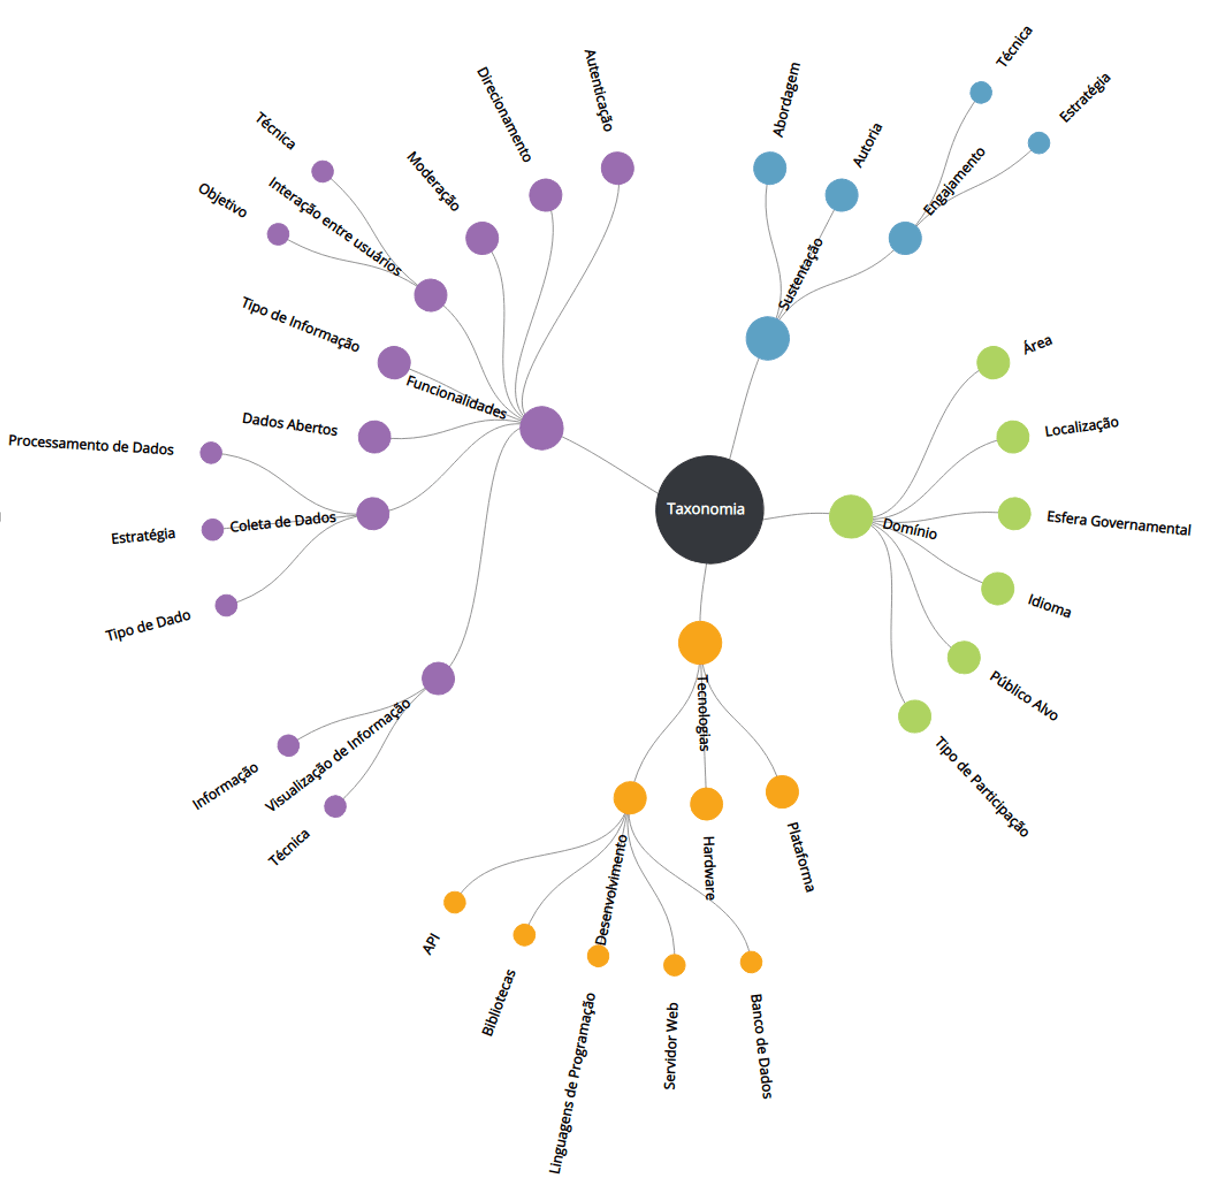
\includegraphics[scale=0.30]{./figuras/taxonopart-radial.png}
    \caption{TAPE. Fonte: \citeonline{tape2019mota}}
    \label{fig:taxonomia-vispublica}
\end{figure}

\subsection{Sustentação}
\label{subsubsec:sustentacao}
O grupo sustentação explora as questões relacionadas a como e quem promove a ferramenta de forma que seja utilizada, ou seja, como se dá a sustentabilidade da ferramenta. 
Na Figura \ref{fig:grupo-sustentacao} é possível observar, isoladamente, a hierarquia para classificação definida no grupo sustentação.

\begin{figure}[!ht]
    \centering
    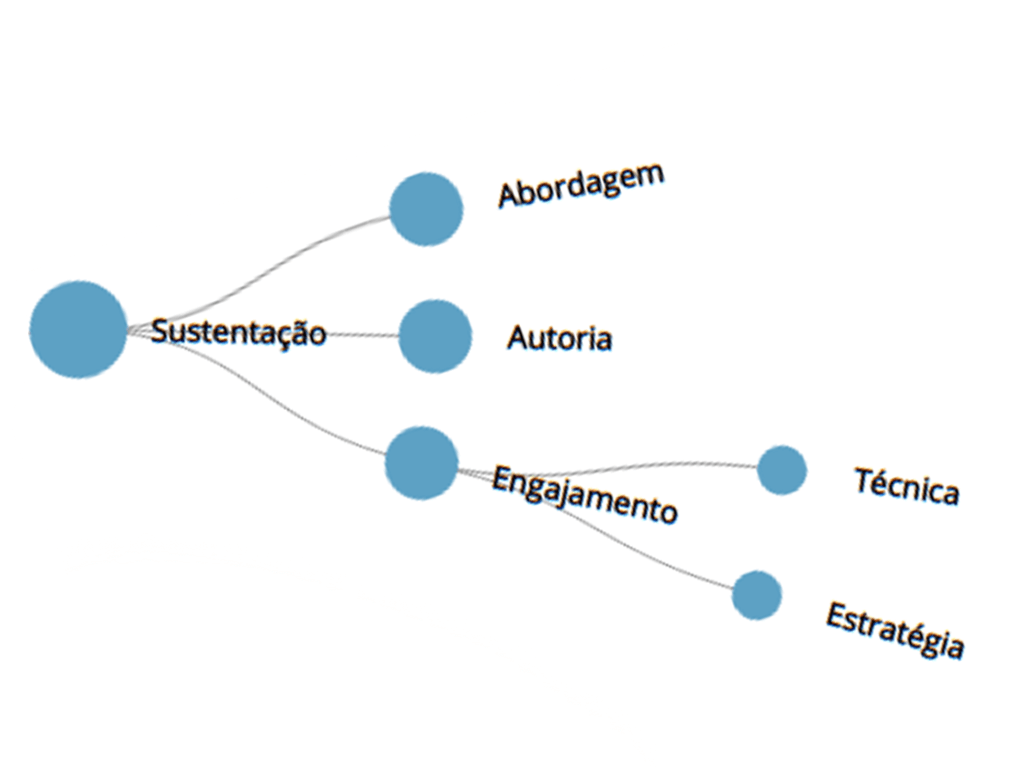
\includegraphics[scale=0.20]{./figuras/sustentacao.png}
    \caption{Hierarquia do grupo sustentação}
    \label{fig:grupo-sustentacao}
\end{figure}

\par
As definições das classe e subclasse desse grupo são representadas e descritas na Tabela \ref{tab:classesSustentacao}.

\begin{table}[!ht]
    \centering
    \caption{Classes e Subclasses do Grupo Sustentação}
    \label{tab:classesSustentacao}
    \begin{tabular}{l*{2}{>{\raggedright\arraybackslash}p{0.3\linewidth}}}
    \toprule
        Nome         & Tipo\\ 
    \midrule
        Abordagem    & Classe\\                         
        Autoria      & Classe\\
        Engajamento  & Classe\\
        Técnica      & Subclasse de Engajamento\\
        Estratégia   & Subclasse de Engajamento\\
    \bottomrule
    \end{tabular}
\end{table}

%========================================================================================================================================================================================
\subsection{Domínio}
\label{subsubsec:dominio}
O grupo domínio tem o objetivo de considerar características do ambiente em que a ferramenta está inserida. 
A figura \ref{fig:grupo-dominio} representa de forma visual as hierarquias definidas para o grupo.

\begin{figure}[!ht]
    \centering
    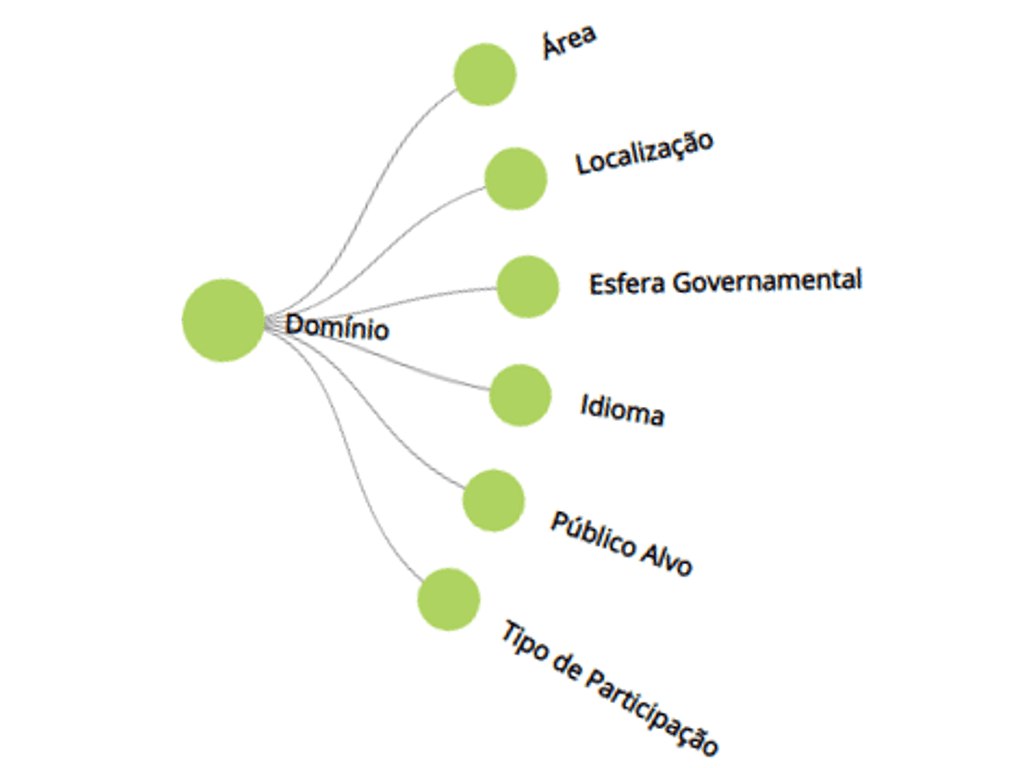
\includegraphics[scale=0.20]{./figuras/dominio.png}
    \caption{Hierarquia do grupo domínio}
    \label{fig:grupo-dominio}
\end{figure}

\par
As definições das classe e subclasse desse grupo são representadas e descritas na Tabela \ref{tab:classesDominio}.

\begin{table}[!ht]
    \centering
    \caption{Classes e Subclasses do Grupo Domínio}
    \label{tab:classesDominio}
    \begin{tabular}{l*{2}{>{\raggedright\arraybackslash}p{0.3\linewidth}}}
    \toprule
        Nome                  & Tipo \\ 
    \midrule
        Área                  & Classe\\      
        Localização           & Classe\\      
        Esfera governamental  & Classe\\      
        Idioma                & Classe\\      
        Público alvo          & Classe\\      
        Tipo de participação  & Classe\\
    \bottomrule
    \end{tabular}
\end{table}

%========================================================================================================================================================================================
\subsection{Tecnologias}
\label{subsubsec:tecnologias}
O grupo tecnologia contempla a análise sobre os aspectos técnicos utilizados nas ferramentas.
A figura \ref{fig:grupo-tecnologias} representa de forma visual as hierarquias definidas para o grupo.

\begin{figure}[!ht]
    \centering
    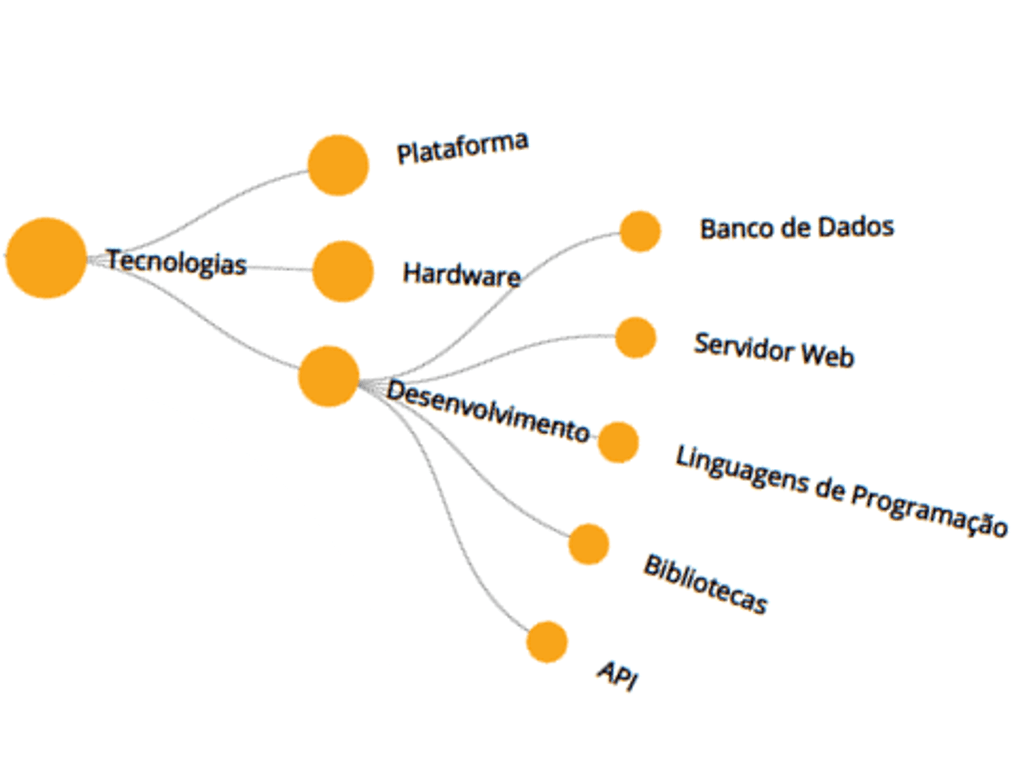
\includegraphics[scale=0.20]{./figuras/tecnologias.png}
    \caption{Hierarquia do grupo tecnologias}
    \label{fig:grupo-tecnologias}
\end{figure}

\par
As definições das classe e subclasse desse grupo são representadas e descritas na Tabela \ref{tab:classesTecnologias}.

\begin{table}[!ht]
    \centering
    \caption{Classes e Subclasses do Grupo Tecnologias}
    \label{tab:classesTecnologias}
    \begin{tabular}{l*{2}{>{\raggedright\arraybackslash}p{0.4\linewidth}}}
    \toprule
        Nome                      & Tipo \\ 
    \midrule
        Plataforma                & Classe\\      
        Hardware                  & Classe\\      
        Desenvolvimento           & Classe\\      
        Banco de dados            & Sublasse de Desenvolvimento\\      
        Servidor web              & Sublasse de Desenvolvimento\\
        Linguagens de Programação & Sublasse de Desenvolvimento\\
        Bibliotecas               & Sublasse de Desenvolvimento\\
        API                       & Sublasse de Desenvolvimento\\
    \bottomrule
    \end{tabular}
\end{table}

%========================================================================================================================================================================================
\subsection{Funcionalidades}
\label{subsubsec:funcionalidades}
O grupo funcionalidades aborda as principais características de utilização disponibilizadas para interação com o usuário.
A hierarquia proposta para o grupo Tecnologias está representada na figura \ref{fig:grupo-funcionalidades}.

\begin{figure}[!ht]
    \centering
    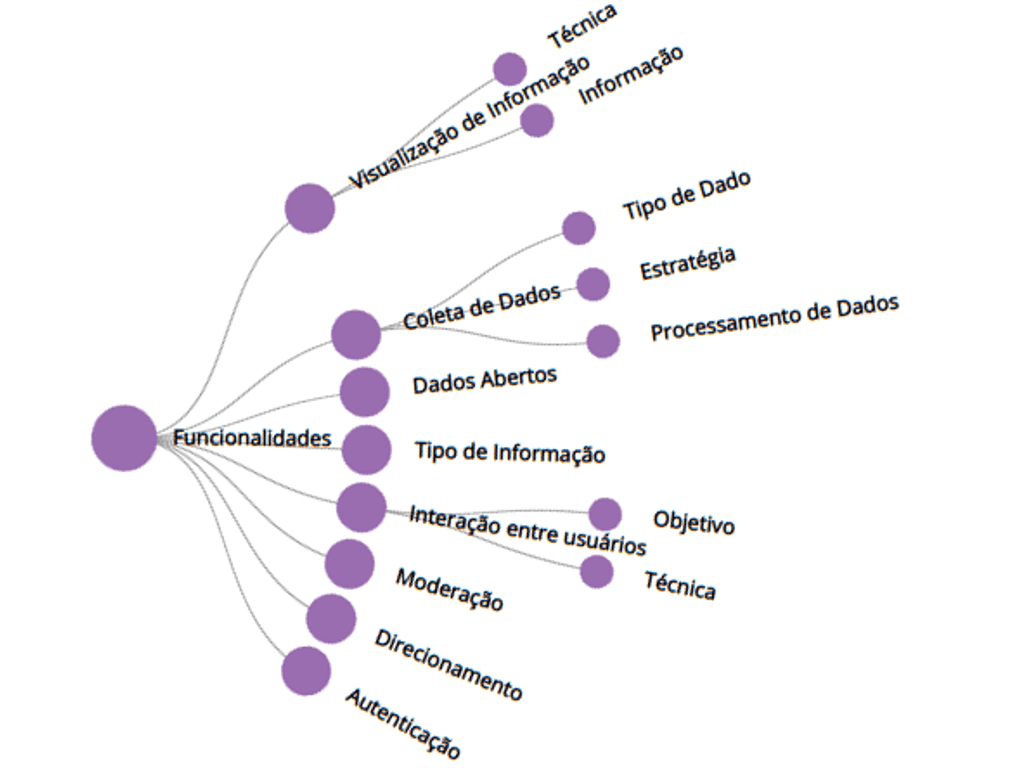
\includegraphics[scale=0.30]{./figuras/funcionalidades.png}
    \caption{Hierarquia do grupo funcionalidades}
    \label{fig:grupo-funcionalidades}
\end{figure}

\par
As definições das classe e subclasse desse grupo são representadas e descritas na Tabela \ref{tab:classesFuncionalidades}.

\begin{table}[!ht]
    \centering
    \caption{Classes e Subclasses do Grupo Funcionalidades}
    \label{tab:classesFuncionalidades}
    \begin{tabular}{l*{2}{>{\raggedright\arraybackslash}p{0.5\linewidth}}}
    \toprule
        Nome                       & Descrição \\ 
    \midrule
        Visualização de Informação & Classe \\
        Técnica                    & Subclasse de Visualização de Informação\\
        Informação                 & Subclasse de Visualização de Informação\\
        Coleta de Dados            & Classe \\
        Tipo de Dado               & Subclasse de Coleta de Dados\\
        Estratégia                 & Subclasse de Coleta de Dados\\
        Processamento de Dados     & Subclasse de Coleta de Dados\\
        Dados abertos              & Classe \\
        Tipo de Informação         & Classe \\
        Interação entre usuários   & Classe \\
        Objetivo                   & Subclasse de Interação entre usuários \\
        Técnica	                   & Subclasse de Interação entre usuários \\
        Moderação                  & Classe \\
        Direcionamento             & Classe \\
        Autenticação               & Classe \\
    \bottomrule
    \end{tabular}
\end{table}

    % Capítulo 3 - Ferramenta
    \chapter[Ferramenta]{Ferramenta}
\label{cap:cap3}

Neste capítulo apresentamos a ferramenta elaborada.

    % Capítulo 4 - Avaliação
    \chapter[Avaliação da Ferramenta]{Avaliação da Ferramenta}
\label{cap:cap4}

Nesse capítulo são apresentadas a metodologia utilizada para avaliação de usabilidade da ferramenta e-TAPE, assim como a a análise dos resultados obtidos.

% 1a seção do capítulo 4
\section{Cenário da Avaliação}
\label{sec:cenario}
O objetivo desta avaliação foi analisar a usabilidade da ferramenta desenvolvida com a utilização por possíveis usuários finais. Essa avaliação foi dividida em três etapas,
sendo a primeira a identificação do perfil dos participantes e apresentação do experimento, a segunda etapa consistem na realização das tarefas pré-determinadas, 
e por último a avaliação da usabilidade da ferramenta.

\par
Na primeira etapa, os participantes foram informados quanto ao objetivo do experimento, orientados sobre os procedimentos a serem seguidos. 
A coleta de dados sobre o perfil foi realizada através de um questionário, descrito na tabela \ref{tab:questionario}. 
O questionário original aplicado aos participantes pode ser encontrado no Anexo \ref{anexo:questionario}.

\begin{table}[!ht]
    \centering
    \caption{Dados coletados  sobre o perfil dos participantes}
    \label{tab:questionario}
    \begin{tabular}{l*{2}{>{\raggedright\arraybackslash}p{0.2\linewidth}}}
    \toprule
        Pergunta        \\
    \midrule
        Qual seu sexo? \\
        Qual sua idade?\\
        Qual seu grau de escolaridade?\\
        Você conhece o conceito de participação eletrônica?\\
        Se respondeu sim na pergunta anterior,\\ por onde conheceu o conceito de participação eletrônica?\\
        Você costuma discutir questões sociais na internet?\\
        Se respondeu sim na pergunta anterior,\\ costuma discutir com: \\
        Caso você discuta questões sociais na internet, qual(is) ferramentas utiliza? \\
        Você sabe o que é uma Taxonomia?\\
    \bottomrule
    \end{tabular}
\end{table}

\par
Após a primeira etapa, foi disponibilizada uma máquina com acesso a internet para que os participantes pudessem acessar a e-TAPE. Foi dado a cada usuário o tempo de cinco minutos para se informar sobre a TAPE, lendo as definições dos grupos, classes e subclasses,
disponíveis na primeira página da aplicação. 
Após os cinco minutos, foi entregue a cada usuário duas descrições textuais sobre ferramentas de participação eletrônica. Essas descrições foram elaboradas pelos pesquisadores envolvidos na construção da TAPE que são especialistas em participação eletrônica. 
A partir dessas descrições, cada usuário deveria classificar a ferramenta descrita usando a e-TAPE de acordo com o que achasse mais adequado.
Essa abordagem foi adotada para que fosse possível a comparação entre a classificação de uma ferramenta de participação feita por um especialista em comparação com a classificação por usuários leigos. O tempo gasto para leitura das descrições textuais e classificação das ferramentas foi cronometrado e registrado.
As descrições de ferramentas apresentadas aos participantes estão disponíveis no Apêndice X deste trabalho.

\par
Na terceira etapa, após finalizada a interação do usuário participante com a ferramenta, o objetivo foi avaliar a usabilidade da ferramenta e-TAPE.
Para essa avaliação, foi utilizado o questionário \acrfull{sus}, desenvolvido por \citeonline{brooke1996sus}, composto de 10 itens \textit{likert}. 
Cada item é associado a uma escala \textit{likert} de 5 pontos, sendo o valor 1 atribuído ao discordo totalmente e o  5 atribuído ao concordo totalmente.
A figura \ref{fig:exemplo-pergunta} exemplifica um item \textit{likert}.

\begin{figure}[!ht]
    \centering
    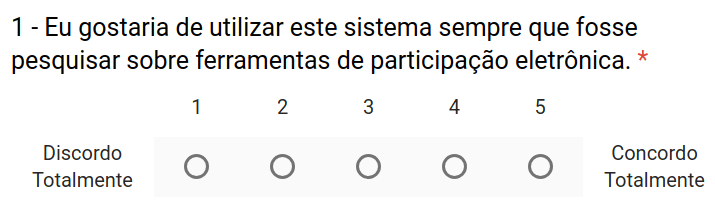
\includegraphics[scale=0.5]{./figuras/exemplo_pergunta.png}
    \caption{Exemplo de um item \textit{Likert}}
    \label{fig:exemplo-pergunta}
\end{figure}

\par
Seguindo a metodologia utilizada por \citeonline{brooke1996sus}, foi solicitado aos participantes que respondessem ao questionário, todos os 10 itens devem ser respondidos,
caso o participante não saiba como responder a algum item em especial, deve-se solicitar que responda-o com o valor três, ao centro da escala. A coleta das respostas, 
deve ser feita imediatamente ao término da leitura de cada item, evitando que se pense muito tempo sobre cada resposta, o autor alega que essa metodologia é robusta e confiável.

\par
As 10 questões que compõem o questionário foram definidas por \citeonline{brooke1996sus}, após a aplicação de um questionário sobre dois sistemas diferentes com 50 itens em potencial. Desses 50 itens, foram selecionados os 5 com os maiores valores de concordância e os outros 5 com maiores valores de discordância. Os 10 itens selecionados
foram postos alternadamente, com o objetivo de evitar respostas automáticas, obrigando o respondente a se esforçar para pensar se concorda ou discorda de cada item. 

\par
O questionário \acrshort{sus} permite o cálculo de um indicador para a usabilidade geral do sistema avaliado, denominado \textit{Score SUS} . 
\citeonline{brooke1996sus} definiu o cálculo do \textit{Score SUS} da seguinte forma:
Para os itens 1, 3, 5, 7 e 9, será o valor assinalado pelo respondente menos 1. Para os itens 2, 4, 6, 8 e 10, será 5 menos o valor assinalado. Após isso, a soma dos valores 
encontrados é multiplicada por 2,5, obtendo-se o \textit{Score SUS} para o sistema avaliado.

\par
O questionário proposto no trabalho original está descrito no Anexo \ref{anexo:questionario} e  foi adaptado ao contexto de utilização da e-TAPE de maneira que as especificidades desse domínio fossem consideradas na avaliação. O questionário utilizado está descrito na Tabela \ref{tab:questionario3}

\begin{table}[!ht]
    \centering
    \caption{Questionário SUS adaptado para avaliação da e-TAPE}
    \label{tab:questionario3}
    \begin{tabular}{l*{2}{>{\raggedright\arraybackslash}p{0.66\linewidth}}}
    \toprule
    Nº & Questão        \\
    \midrule
    1 & Eu gostaria de utilizar este sistema sempre que fosse pesquisar sobre ferramentas de participação eletrônica.\\
    2 & Eu achei a aplicação desnecessariamente complexa. \\
    3 & Eu achei a aplicação fácil de usar.\\
    4 & Eu acho que precisaria de apoio de um suporte técnico para ser possível interagir com essa aplicação.\\
    5 & Eu achei que as diversas funções nesta aplicação foram bem integradas. \\
    6 & Eu achei que houve muita inconsistência ou erros nesta aplicação. \\
    7 & Eu imaginaria que a maioria das pessoas, interessadas em ferramentas de participação eletrônica, aprenderia a usar essa aplicação rapidamente. \\
    8 & Eu achei a aplicação muito complicada. \\
    9 & Eu me senti muito confiante quanto às interações com essa aplicação. \\
    10 & Eu precisei aprender muitas coisas sobre ferramentas de participação eletrônica para que eu pudesse fazer uso da aplicação.\\
    \bottomrule
    \end{tabular}
\end{table}


\par
\citeonline{boucinha2013avaliaccao} afirmam que as questões do \acrshort{sus} podem ser associadas aos componentes de qualidade descritos por \citeonline{nielsen199510},
da seguinte forma:

\begin{table}[!ht]
    \centering
    \caption{Componentes de qualidade de \citeonline{nielsen199510} x Questões \acrshort{sus}}
    \label{tab:componentesQualidadePorQuestao}
    \begin{tabular}{l*{2}{>{\raggedright\arraybackslash}p{0.2\linewidth}}}
    \toprule
        Componente de Qualidade & Questão(ões)        \\
    \midrule
        Facilidade de aprendizagem & 3, 4, 7 e 10 \\
        Eficiência & 5, 6 e 8 \\
        Facilidade de memorização & 2 \\
        Minimização dos erros & 6 \\
        Satisfação & 1, 4 e 9\\
    \bottomrule
    \end{tabular}
\end{table}

\par 
De acordo com os autores, para avaliar cada componente de qualidade, deve-se fazer a média dos valores encontrados durante o cálculo do \textit{Score SUS} para o grupo de perguntas 
em questão \cite{nielsen199510}. Os resultados encontrados foram analisado e estão descritos na Seção \ref{sec:resultados}. 

\section{Resultados}
\label{sec:resultados}

Participaram 12 voluntários no experimento, sendo 75\% do sexo masculino e 25\% do sexo feminino, como apresentado no gráfico da Figura \ref{fig:grafico-sexo}. Além disso, 
é possível observar, pela Figura \ref{fig:grafico-idade}, que a maioria dos participantes tem entre 21 e 25 anos de idade e 
estão com a graduação atualmente em curso, como representado na Figura \ref{fig:grafico-grau}.

\begin{figure}[!ht]
    \centering
    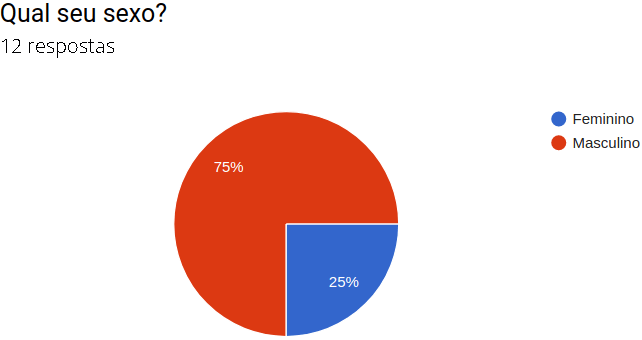
\includegraphics[scale=0.4]{./figuras/sexo.png}
    \caption{Sexo dos participantes}
    \label{fig:grafico-sexo}
\end{figure}

\begin{figure}[!ht]
    \centering
    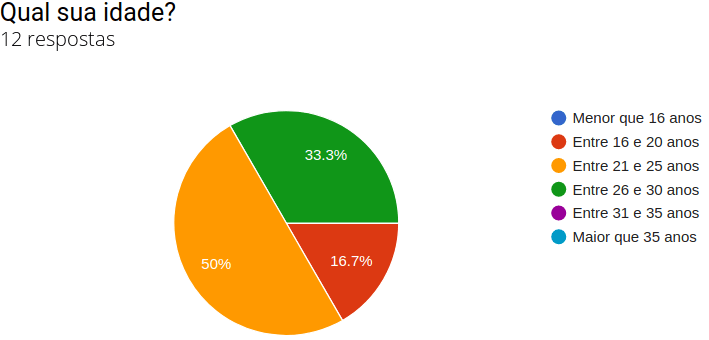
\includegraphics[scale=0.4]{./figuras/idade.png}
    \caption{Idade dos participantes}
    \label{fig:grafico-idade}
\end{figure}

\begin{figure}[!ht]
    \centering
    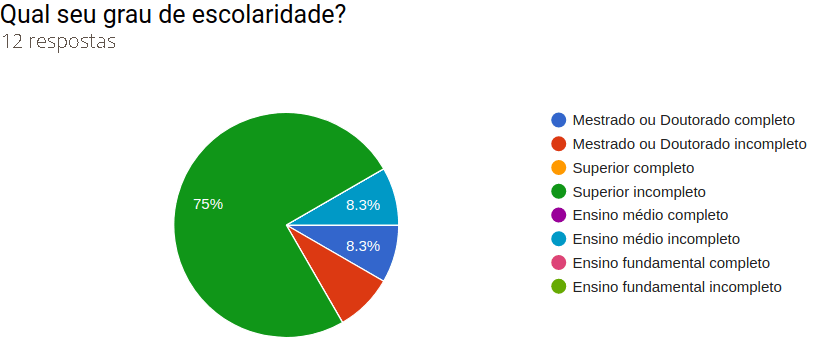
\includegraphics[scale=0.4]{./figuras/grau_escolaridade.png}
    \caption{Grau de escolaridade dos participantes}
    \label{fig:grafico-grau}
\end{figure}

\par
Pôde-se perceber que a maioria dos participantes, 91,7\%, não conhecia o conceito de participação eletrônica, resultado descrito na Figura \ref{fig:grafico-participacao}.

\begin{figure}[!ht]
    \centering
    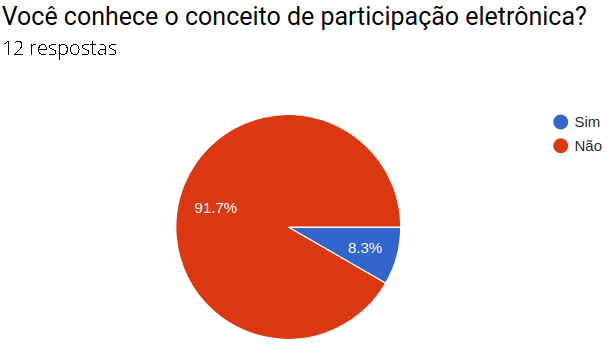
\includegraphics[scale=0.4]{./figuras/conhece_participacao_eletronica.png}
    \caption{Conhecimento sobre o conceito de participação eletrônica dos participantes}
    \label{fig:grafico-participacao}
\end{figure}

\par
Contudo, 58,3\% dos participantes, como observado na Figura \ref{fig:grafico-discu-alvo}, responderam que costumam discutir questões sociais na internet. 
Desses, 80,0\% disseram que  discutem com amigos, colegas ou conhecidos, 20,0\% discutem com amigos, colegas ou conhecidos e desconhecidos, representados pela legenda ambos
no gráfico da figura \ref{fig:grafico-discu-alvo}, ninguém respondeu que discute apenas com desconhecidos. Quando perguntados sobre quais ferramentas de participação 
eletrônica eles utilizam para discutir esse tipo de questão, 100\% das respostas foram redes sociais. 

\begin{figure}[!ht]
    \centering
    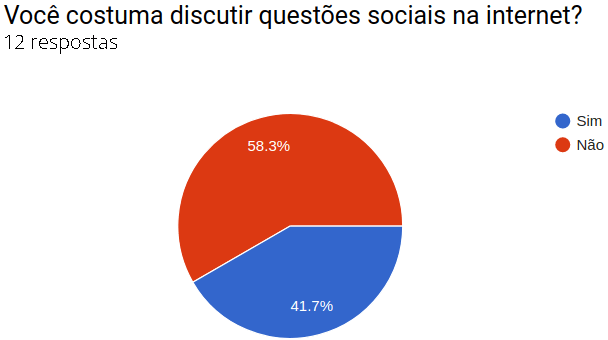
\includegraphics[scale=0.4]{./figuras/discutir.png}
    \caption{Participantes que discutem questões sociais na internet}
    \label{fig:grafico-discu}
\end{figure}

\par
Esse resultado sugere que a discussão sobre questões sociais é importante para os respondentes. Essa característica dos participantes pode ser um indicativo de que a amostra 
considerada tem uma afinidade com o tema investigado uma vez que as ferramentas classificadas estão inseridas nesse universo da participação sendo mediada pelas \acrshort{tic}. 

\begin{figure}[!ht]
    \centering
    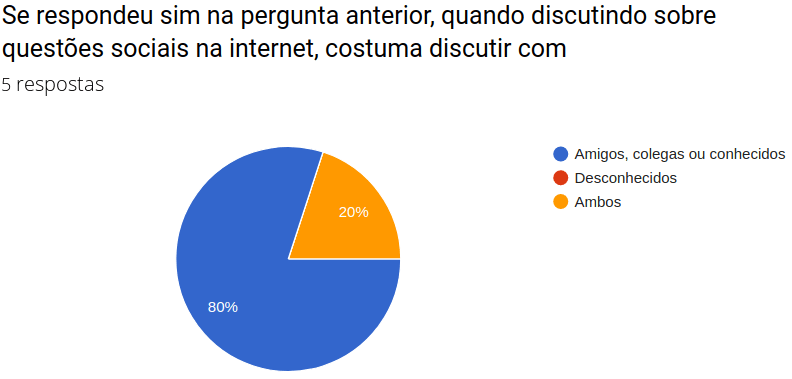
\includegraphics[scale=0.4]{./figuras/discutir_com.png}
    \caption{Pessoas com as quais os participantes que discutem questões sociais na internet interagem.}
    \label{fig:grafico-discu-alvo}
\end{figure}

\par
Quanto a última pergunta da primeira etapa, sobre o conhecimento do conceito de Taxonomia, percebeu-se que a grande maioria, 83,3\% não conhecia esse conceito conforme ilustrado na 
Figura \ref{fig:grafico-conhe-taxonomia}. Esse resultado pode ser um indicativo que mesmo a taxonomia sendo um modelo de classificação antigo, 
não faz parte do escopo de conhecimentos gerais de algumas pessoas.

\begin{figure}[!ht]
    \centering
    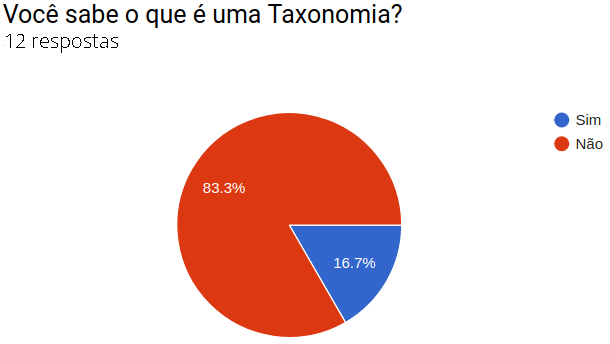
\includegraphics[scale=0.4]{./figuras/sabe_taxonomia.png}
    \caption{Conhecimento do conceito de taxonomia pelos participantes.}
    \label{fig:grafico-conhe-taxonomia}
\end{figure}

\par
O tempo médio dos participantes para a conclusão da classificação das duas ferramentas solicitadas foi de 24 minutos e 16 segundos, o gráfico na Figura \label{fig:grafico-tempo}
representa o tempo gasto por cada participante. Notou-se que participantes que tinham conhecimento prévio sobre ferramentas de participação realizaram 
as tarefas em um tempo 50\% menor se comparado aqueles que não tinham esse tipo de conhecimento.

\par 
O \textit{Score SUS} da aplicação e-TAPE foi de 78,75\%. A Tabela \ref{tab:resultado-questionario} apresenta a média de pontuação de cada item do questionário \acrshort{sus}.

\begin{table}[!ht]
    \centering
    \caption{\textit{Score SUS} de cada item do questionário aplicado}
    \label{tab:resultado-questionario}
    \begin{tabular}{l*{3}{>{\raggedright\arraybackslash}p{0.66\linewidth}p{0.1\linewidth}}}
    \toprule
    Nº & Questão & \textit{Score}    \\
    \midrule
    1 & Eu gostaria de utilizar este sistema sempre que fosse pesquisar sobre ferramentas de participação eletrônica. & ::X \\
    2 & Eu achei a aplicação desnecessariamente complexa. & ::X \\
    3 & Eu achei a aplicação fácil de usar. & ::X \\
    4 & Eu acho que precisaria de apoio de um suporte técnico para ser possível interagir com essa aplicação. & ::X \\
    5 & Eu achei que as diversas funções nesta aplicação foram bem integradas.  & ::X \\
    6 & Eu achei que houve muita inconsistência ou erros nesta aplicação.  & ::X \\
    7 & Eu imaginaria que a maioria das pessoas, interessadas em ferramentas de participação eletrônica, aprenderia a usar essa aplicação rapidamente. & ::X \\
    8 & Eu achei a aplicação muito complicada.  & ::X \\
    9 & Eu me senti muito confiante quanto às interações com essa aplicação.  & ::X \\
    10 & Eu precisei aprender muitas coisas sobre ferramentas de participação eletrônica para que eu pudesse fazer uso da aplicação. & ::X \\
    \bottomrule
    \end{tabular}
\end{table}

\par
A Tabela \ref{tab:resultado-componentes} apresenta o resultado dos componentes de qualidade do \textit{software}. Sendo assim possível chegar a conclusão, pela metodologia aplicada, 
que a ferramenta e-TAPE satisfaz os critérios de qualidade propostos por \citeonline{nielsen199510}, de facilidade de aprendizagem, eficiência, facilidade de memorização,
minimização dos erros e satisfação.

\begin{table}[!ht]
    \centering
    \caption{Valor encontrado para cada componente de avaliação da qualidade da ferramenta e-TAPE}
    \label{tab:resultado-componentes}
    \begin{tabular}{l*{2}{>{\raggedright\arraybackslash}p{0.1\linewidth}}}
        \toprule
            Componente de Qualidade & Valor         \\
        \midrule
            Facilidade de aprendizagem & ::X \\
            Eficiência & ::X \\
            Facilidade de memorização & ::X \\
            Minimização dos erros & ::X \\
            Satisfação & ::X\\
        \bottomrule
        \end{tabular}
\end{table}
    % Capítulo 5 - Conclusão
    \chapter[Conclusão e Trabalhos Futuros]{Conclusão e Trabalhos Futuros}
\label{cap:cap5}

Neste trabalho, foi desenvolvida uma aplicação \textit{web} com o intuito de servir como meio para a edição colaborativa de uma taxonomia
sobre ferramentas de participação eletrônica. Essa taxonomia em questão foi elaborada e denominada como TAPE por \citeonline{tape2019mota}. 
O desenvolvimento da ferramenta e-TAPE é um projeto que se encontra em andamento, e o objetivo deste trabalho foi a construção de uma primeira versão útil dessa aplicação, 
de modo que o projeto pudesse continuar sua evolução.

\par
Como já abordado na seção \ref{sec:desenvolvimento}, a utilização do modelo interativo de desenvolvimento permite que requisitos sejam propostos e avaliados para serem
implementados em futuras versões. A versão atualmente disponível da e-TAPE foi avaliada, através de um questionário SUS, e obteve um \textit{Score SUS}, referente a análise de usabilidade,
de 78,75 em uma escala entre 0 e 100. O autor \citeonline{sauro2015supr} estabelece uma média de 68 pontos como referência para a avaliação de ferramentas. 
Assim, constata-se que para uma primeira versão, e-TAPE conseguiu atingir uma boa avaliação. 

\par
A avaliação também gerou dados sobre os componentes de avaliação da qualidade da ferramenta, onde a e-TAPE ficou acima da média em 3 dos 5 critérios de avaliação. Com isso foram
identificadas algumas limitações, mas o resultado, de maneira geral, foi satisfatório. 

\par
Além das funcionalidades associadas à facilidade de uso e satisfações identificadas na avaliação, outras funcionalidades já estão previstas para serem implementadas, como: 
permitir o cadastro e o controle de acesso por diferente classes de usuários (moderadores, cidadãos e visitantes), permitir a edição da taxonomia de forma moderada, 
integração com redes sociais para compartilhamento e adição de comentários e sugestão de evolução da taxonomia. 


\par
Espera-se que este projeto e a aplicação e-TAPE contribua com pesquisadores, gestores públicos e sociedade civil para que as iniciativas de ferramentas de participação eletrônica
sejam amplamente difundidas e utilizadas. 


    
    % Elementos pós-textuais
    \postextual
    % Apêndices - opcional
    \apendices
    %\partapendices 	% imprime uma página indicando o início dos apêndices
    \chapter{Resultados do questionário}
\label{apendice:a}

\begin{figure}[!ht]
    \centering
    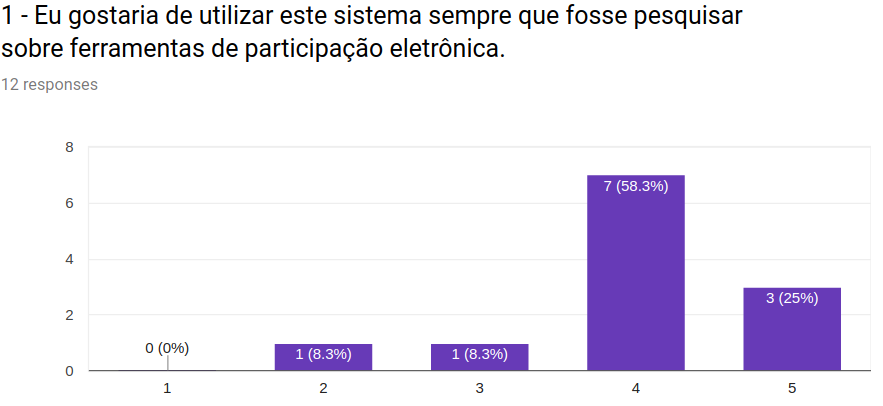
\includegraphics[scale=0.5]{./figuras/q1.png}
    \caption{Resultado do item 1.}
    \label{fig:q1}
\end{figure}

\begin{figure}[!ht]
    \centering
    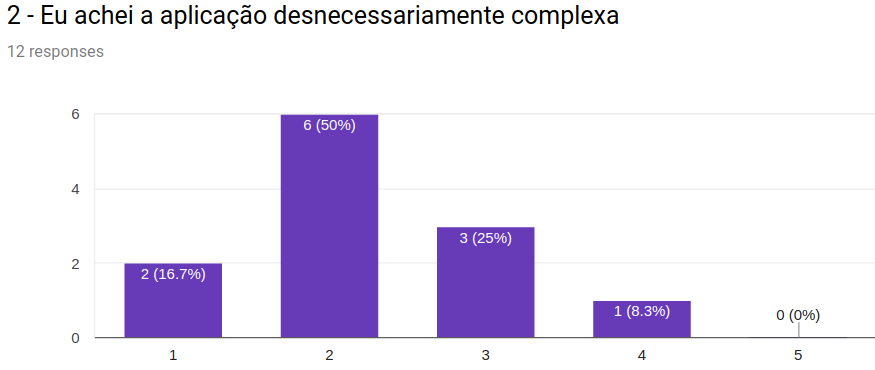
\includegraphics[scale=0.5]{./figuras/q2.png}
    \caption{Resultado do item 2.}
    \label{fig:q2}
\end{figure}

\begin{figure}[!ht]
    \centering
    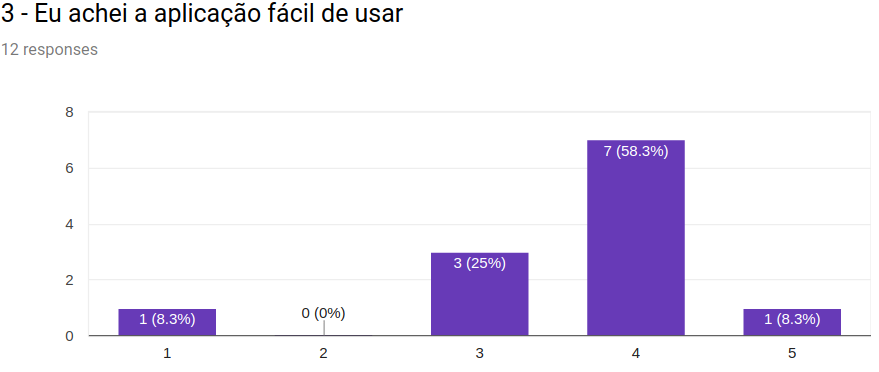
\includegraphics[scale=0.5]{./figuras/q3.png}
    \caption{Resultado do item 3.}
    \label{fig:q3}
\end{figure}

\begin{figure}[!ht]
    \centering
    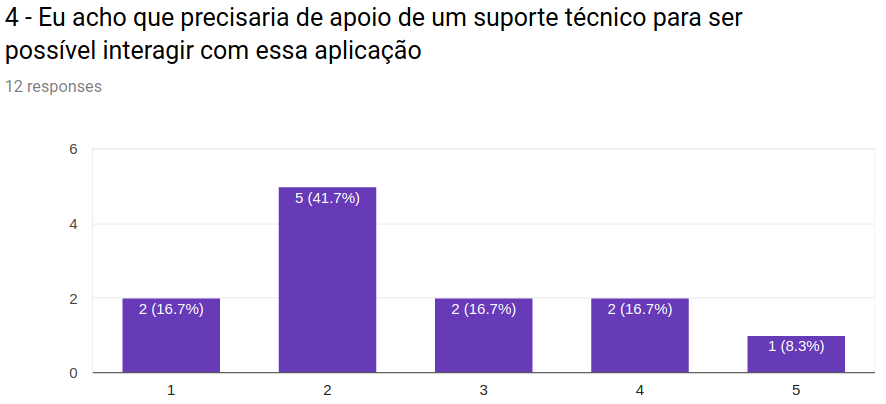
\includegraphics[scale=0.5]{./figuras/q4.png}
    \caption{Resultado do item 4.}
    \label{fig:q4}
\end{figure}

\begin{figure}[!ht]
    \centering
    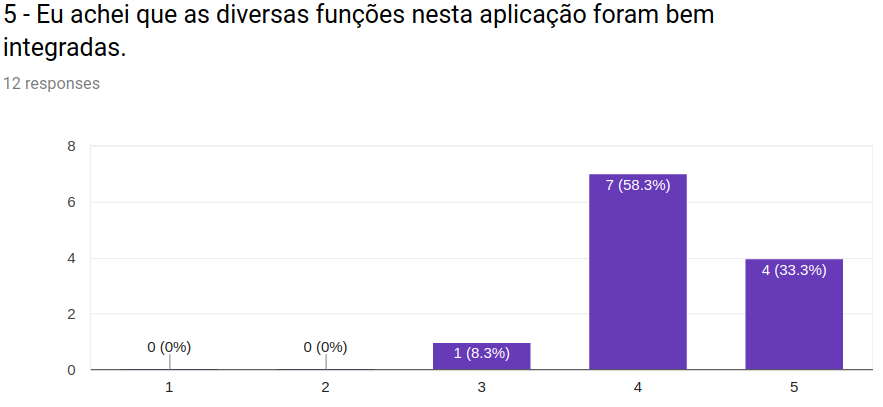
\includegraphics[scale=0.5]{./figuras/q5.png}
    \caption{Resultado do item 5.}
    \label{fig:q5}
\end{figure}

\begin{figure}[!ht]
    \centering
    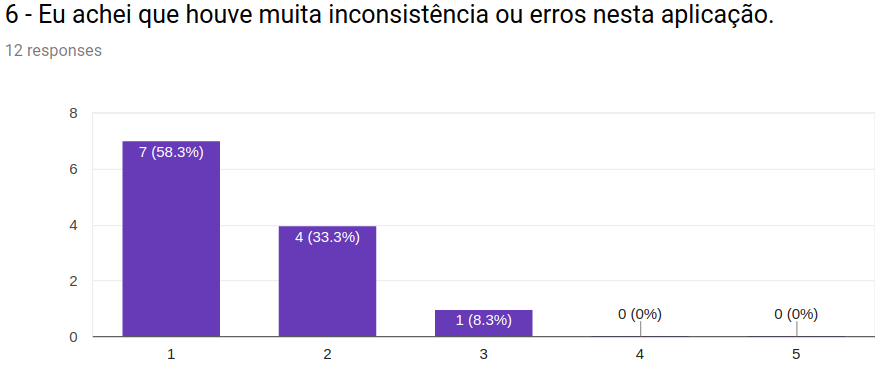
\includegraphics[scale=0.5]{./figuras/q6.png}
    \caption{Resultado do item 6.}
    \label{fig:q6}
\end{figure}

\begin{figure}[!ht]
    \centering
    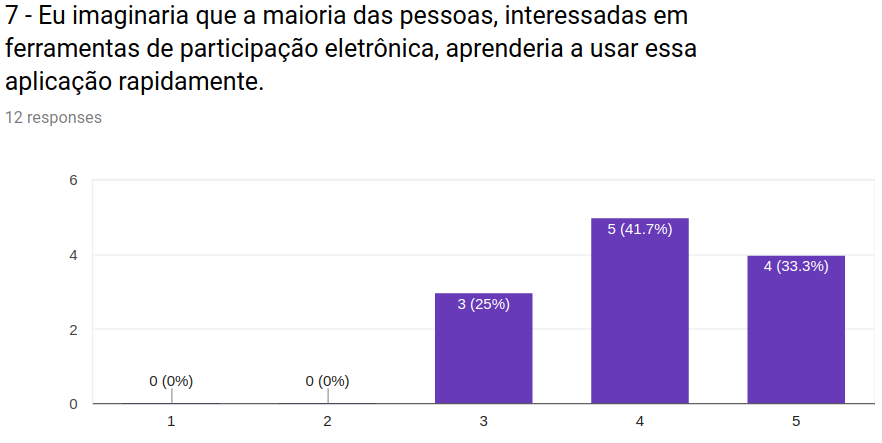
\includegraphics[scale=0.5]{./figuras/q7.png}
    \caption{Resultado do item 7.}
    \label{fig:q7}
\end{figure}

\begin{figure}[!ht]
    \centering
    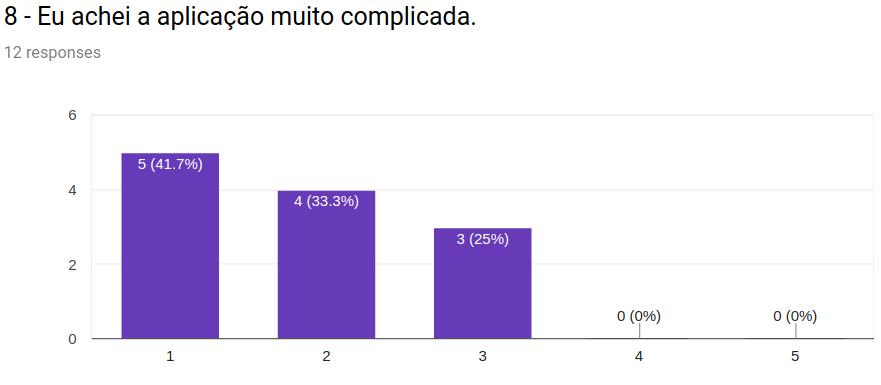
\includegraphics[scale=0.5]{./figuras/q8.png}
    \caption{Resultado do item 1.}
    \label{fig:q8}
\end{figure}

\begin{figure}[!ht]
    \centering
    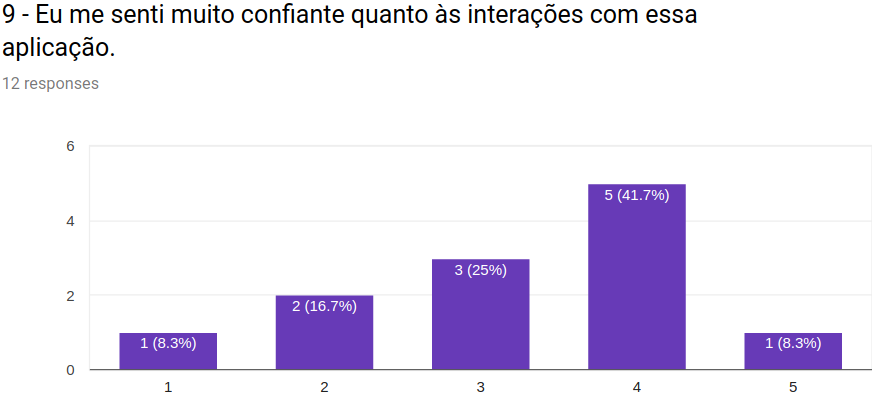
\includegraphics[scale=0.5]{./figuras/q9.png}
    \caption{Resultado do item 9.}
    \label{fig:q9}
\end{figure}

\begin{figure}[!ht]
    \centering
    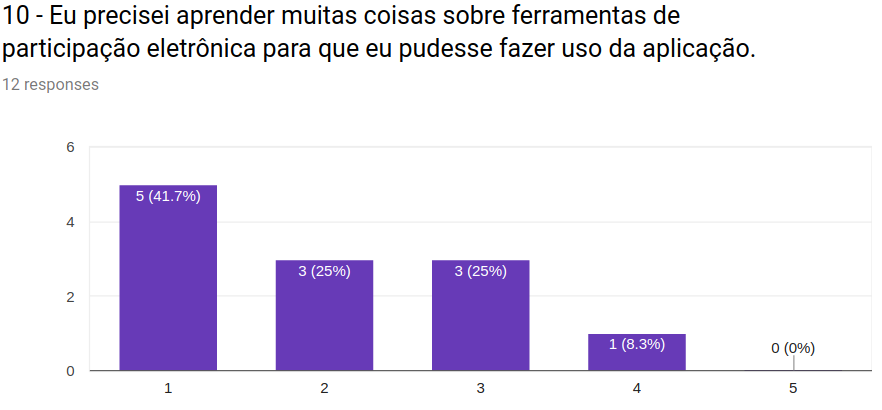
\includegraphics[scale=0.5]{./figuras/q10.png}
    \caption{Resultado do item 10.}
    \label{fig:q10}
\end{figure}
    \chapter{Lista de Requisitos}
\label{apendice:b}

\begin{itemize}
    \item [RFS001] – Inserir Usuário
    \item [RFS002] – Visualizar/Listar Usuário
    \item [RFS003] – Alterar Usuário
    \item [RFS004] – Remover Usuário
    \item [RFS005] – Inserir Taxonomia
    \item [RFS006] – Visualizar Taxonomia
    \item [RFS007] – Alterar Taxonomia
    \item [RFS008] – Remover Taxonomia
    \item [RFS009] – Visualizar/Listar VersãoTaxonomia
    \item [RFS010] – Inserir Permissão de Usuário
    \item [RFS011] – Visualizar/Listar Permissões de Usuário 
    \item [RFS012] – Alterar Permissão de Usuário
    \item [RFS013] – Remover Permissão de Usuário
    \item [RFS014] – Inserir Ferramenta
    \item [RFS015] – Visualizar/Listar Ferramentas
    \item [RFS016] – Alterar Ferramenta
    \item [RFS017] – Remover Ferramenta
    \item [RFS018] – Inserir Árvore Taxonômica
    \item [RFS019] – Visualizar Árvore Taxonômica
    \item [RFS020] – Alterar Árvore Taxonômica
    \item [RFS021] – Remover Árvore Taxonômica
    \item [RFS022] – Inserir Classificação
    \item [RFS023] – Visualizar/Listar Classificação
    \item [RFS024] – Alterar Classificação
    \item [RFS025] – Remover Classificação
    \item [RFS026] – Visualizar/Listar Tutoriais
    \item [RNF001] – Confiabilidade
    \item [RNF002] – Disponibilidade
    \item [RNF003] – Segurança
    \item [RNF004] – Manutenção
    \item [RNF005] – Portabilidade
\end{itemize}
    \chapter{Descrição das ferramentas entregue aos participantes do estudo.}
\label{apendice:c}

\par
Neste apêndice encontram-se os textos submetidos como tarefa aos participantes do estudo.

\section{Texto 1}
\label{sec:text1}
Colab.re

Colab.re é uma ferramenta de participação eletrônica construída como uma rede social na tentativa de aumentar a quantidade de usuários, consequentemente a participação e o engajamento. 
Na ferramenta,  os usuários podem se cadastrar e se inscrever em determinadas cidades para visualizar e inserir problemas. Não podem ser inseridos problemas das esferas estaduais, 
regionais e federais, somente municipais. Na inserção do problema, é possível adicionar vários tipos de dados, como foto, a localização e uma descrição textual. Isso é feito através
de um formulário disponibilizado na própria página da ferramenta. Os usuários visualizam os problemas inseridos na cidade e podem se comunicar através de mensagens de texto com outros
usuários para discutir os problemas e propor soluções. A ferramenta também  disponibiliza módulos específicos para os gestores que podem responder usuários, criar enquetes, 
visualizar os problemas cadastrados em mapas e outros gráficos. A ferramenta é divulgada no Facebook e em um blog no qual são disponibilizados conteúdos sobre participação
cidadã e novidades da ferramenta. Essa estratégia é usada para aumentar o engajamento da ferramenta. A rede social está disponível online  em www.colab.re ou por
aplicativos móveis. A ferramenta foi construída, tanto para plataforma web quanto para mobile, utilizando as seguintes tecnologias: o banco de dados MongoDB, a linguagem de 
programação Javascript junto das bibliotecas Jquery, Angular, MomentJs, Highcharts e Modernizr. Além de contar com consumo de serviços de APIs do Google Maps e Facebook. 
Sabe-se que a ferramenta é hospedada em servidores que utiliza tecnologias como Node.js e Nginx. Os recursos da ferramenta são disponibilizados tanto em português quanto em inglês. 

\section{Texto 2}
\label{sec:text2}

Triang

Triang é uma ferramenta de participação eletrônica iniciada pela comunidade e orientada ao governo, a ferramenta foi criada pela Triang Inc. Com o intuito de aumentar engajamento dos
usuários, usou-se a técnica de gamificação. Para pontuar no jogo, o cidadão deve cadastrar problemas encontrados pela cidade, onde outros usuários podem interagir com ele, propondo
soluções aos problemas encontrados. Para cadastrar um problema, o usuário deve fazer login utilizando alguma rede social. Os jogadores são ranqueados, com a intenção de criar-se uma 
competição entre os jogadores, e assim, aumentar seu engajamento na ferramenta. Na inserção do problema, é possível adicionar vários tipos de dados, como foto, vídeo, a localização e 
uma descrição. Isso é feito através de um dispositivo móvel. Os usuários são notificados de problemas adicionados a 30km de sua localização. Há uma moderação dos problemas inseridos. 
Caso um problema receba avaliação negativa dos outros usuários, é alertado ao moderador para uma revisão do conteúdo. 
A ferramenta também disponibiliza módulos especiais para os gestores  públicos que podem responder aos usuários, criar enquetes, visualizar os problemas cadastrados em mapas e outros 
gráficos. Há a disponibilização das informações geradas abertamente à comunidade. 
A ferramenta é divulgada no Facebook, twitter e instagram, além de um canal no Youtube, onde é possível encontrar tutoriais para aprender a interagir com a ferramenta..
A ferramenta foi construída, somente para plataforma web, utilizando as seguintes tecnologias: o banco de dados PostgreSQL, a linguagem de programação Java junto das bibliotecas
Primefaces, Jquery, D3js e materialize. Além de contar com consumo de serviços de APIs do Google+, linkedin e Facebook. Sabe-se que a ferramenta é hospedada em servidores Wildfly. 
Os recursos da ferramenta são disponibilizados tanto em português, inglês, espanhol e alemão.

    % Anexos - opcional
    \anexos
    %\partanexos		% imprime uma página indicando o início dos anexos
    \chapter{Questionário SUS utilizado como referência ao aplicado aos participantes}
\label{anexo:questionario}

\begin{enumerate}
    \item I think that I would like to use this system frequently.
    \item I found the system unnecessarily complex.
    \item I thought the system was easy to use.
    \item I think that I would need the support of a technical person to be able to use this system.
    \item I found the various functions in this system were well integrated.
    \item I thought there was too much inconsistency in this system
    \item I would imagine that most people would learn to use this system very quickly
    \item I found the system very cumbersome to use.
    \item I felt very confident using the system.
    \item I needed to learn a lot of things before I could get going  with this system
\end{enumerate}
    
    \phantompart	% adiciona espaço no sumário
    % Referências bibliográficas - obrigatório
    \bibliographystyle{abntex2-alf}
    \bibliography{bibliografia.bib}
    % Índice remissivo - opcional
    \printindex	% imprime as páginas nas quais as macros \index{palavra a ser indexada} apareceram.
    
    % Fim do documento
    \end{document}